\documentclass[12pt,fleqn]{article}\usepackage{../common}
\begin{document}
Banglades'te su kuyusu degisiminin lojistik modeli

Bu analiz Gelman ve Hill'in kitabi {\em Data Analysis Using Regression and
Multilevel/Hierarchical Models} 5.4'uncu bolumu isliyor.

Verimizde 3,000 haneye gidilerek anketle toplanmis veri var. Veride
hanelerin yakinlarindaki kuyudaki arsenik seviyesi toplanmis, ve
paylasilan verideki tum hanelerin kuyular sagliksiz seviyede arsenik
iceriyor. Verideki diger bilgiler en yakindaki "saglikli" bir kuyuya
yakinlik, ve o hanenin bu saglikli su kuyusuna (bir sene sonra yapilan
kontrole gore) gecip gecmedigi.  Ayrica hanede fikri sorulan kisinin
egitim seviyesi ve bu hanedeki kisilerin herhangi bir sosyal topluluga
(community assocation) ait olup olmadiklari.

Amacimiz su kuyusunun degisimini modellemek. Bu eylem olup / olmama baglaminda
evet / hayir seklinde bir degisken oldugu icin ikili (binary) olarak
temsil edilebilir ve ikili cevaplar / sonuclar lojistik regresyon ile
modellenebilirler.

Veriye bakalim.

\begin{minted}{python}
from pandas import *
from statsmodels.formula.api import logit
from patsy import dmatrix, dmatrices
\end{minted}

\begin{minted}{python}
df = read_csv('wells.dat', sep = ' ', header = 0, index_col = 0)
print df.head()
\end{minted}

\begin{verbatim}
   switch  arsenic       dist  assoc  educ
1       1     2.36  16.826000      0     0
2       1     0.71  47.321999      0     0
3       0     2.07  20.966999      0    10
4       1     1.15  21.486000      0    12
5       1     1.10  40.874001      1    14
\end{verbatim}

Model 1: Guvenli su kuyusuna uzaklik

Ilk once modelde kuyu uzakligini kullanalim. 

\begin{minted}{python}
model1 = logit("switch ~ dist", df).fit()
print model1.summary()
\end{minted}

\begin{verbatim}
Optimization terminated successfully.
         Current function value: 0.674874
         Iterations 4
                           Logit Regression Results                           
==============================================================================
Dep. Variable:                 switch   No. Observations:                 3020
Model:                          Logit   Df Residuals:                     3018
Method:                           MLE   Df Model:                            1
Date:                Tue, 03 Dec 2013   Pseudo R-squ.:                 0.01017
Time:                        10:24:50   Log-Likelihood:                -2038.1
converged:                       True   LL-Null:                       -2059.0
                                        LLR p-value:                 9.798e-11
==============================================================================
                 coef    std err          z      P>|z|      [95.0% Conf. Int.]
------------------------------------------------------------------------------
Intercept      0.6060      0.060     10.047      0.000         0.488     0.724
dist          -0.0062      0.001     -6.383      0.000        -0.008    -0.004
==============================================================================
\end{verbatim}

Uzaklik (dist) icin elde edilen katsayi -0.0062, fakat bu sayi kafa
karistirici olabilir cunku uzaklik metre olarak olculur, o zaman bu
katsayi mesela 90 metre ile 91 metre uzakligin degisime olan etkisini
olcmektedir, kisacasi pek faydali degildir. Yani uzaklik metre ile
olculdugu icin 1 metrenin modeldeki etkisi ufak, o yuzden bu olcutu
olceklersek (scale) belki regresyon katsayilarimiz daha net
cikar.

Bunu nasil yapacagiz?  Olceklenmis yeni bir degisken yaratmak yerine,
onu formulun icinde tanimlayabiliriz.  Burada bir ara not: eger formul
icinde +,- gibi operasyonlari aritmetik islem olarak kullanmak
istiyorsak, o zaman 'I()' cagrisini yapmak lazim, cunku + operasyonu
mesela Patsy formullerinde baska amaclar icin kullaniliyor. 'I' harfi
birim (identity) kelimesinden geliyor, yani hicbir seyin degismedigini
anlatmaya ugrasiyoruz, "icinde ne varsa onu ver" diyoruz [1].

\begin{minted}{python}
model1 = logit('switch ~I(dist/100.)', df).fit()
print model1.summary()
\end{minted}

\begin{verbatim}
Optimization terminated successfully.
         Current function value: 0.674874
         Iterations 4
                           Logit Regression Results                           
==============================================================================
Dep. Variable:                 switch   No. Observations:                 3020
Model:                          Logit   Df Residuals:                     3018
Method:                           MLE   Df Model:                            1
Date:                Tue, 03 Dec 2013   Pseudo R-squ.:                 0.01017
Time:                        10:24:54   Log-Likelihood:                -2038.1
converged:                       True   LL-Null:                       -2059.0
                                        LLR p-value:                 9.798e-11
==================================================================================
                     coef    std err          z      P>|z|      [95.0% Conf. Int.]
----------------------------------------------------------------------------------
Intercept          0.6060      0.060     10.047      0.000         0.488     0.724
I(dist / 100.)    -0.6219      0.097     -6.383      0.000        -0.813    -0.431
==================================================================================
\end{verbatim}

Simdi modelimizi grafikleyelim. Yanliz degisim (switch) verisini suni olarak
kaydirmamiz / segirtmemiz (jitter) gerekiyor, cunku degisim 0 ve 1'den baska
bir sey olamaz ve grafik surekli ayni iki bolgeye nokta basip duracak. 

\begin{minted}{python}
def binary_jitter(x, jitter_amount = .05):
    '''
    0/1 vektoru iceren veriye segirtme ekle
    '''
    jitters = np.random.rand(*x.shape) * jitter_amount
    x_jittered = x + np.where(x == 1, -1, 1) * jitters
    return x_jittered

plt.plot(df['dist'], binary_jitter(df['switch'], .1), '.', alpha = .1)
plt.plot(np.sort(df['dist']), model1.predict()[np.argsort(df['dist'])], lw = 2)
plt.ylabel('Switched Wells')
plt.xlabel('Distance from safe well (meters)')
plt.savefig('wells_1.png')
\end{minted}

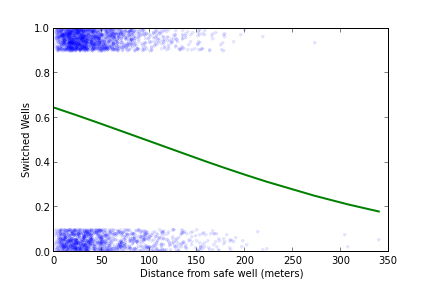
\includegraphics[height=5cm]{wells_1.png}


Mavi noktalar gercek veri, yesil cizgi ise uzaklik gecilerek modelin
olusturdugu "tahmin". Modelin gercek veriye ne kadar uydugunu
goruyoruz boylece, yesil cizginin yuksek olasilik verdigi bolgelerde
ust kismin daha mavi olmasini bekleriz mesela. Ustteki resimde asagi
yukari bunu gosteriyor.

Bir problemin grafiklemesine baska bir yonden yaklasalim, kuyu
degistirenlerin degisim uzakliginin yogunlugu, bir de kuyu
degistirmeyenlerin degisim uzakliginin yogunlugu. Degisimi yapanlarin
dagilimina bakinca, kisa mesafelerde daha fazla yogunluk gormeyi bekliyoruz,
degistirmeyenlerin ise uzun mesafelerde daha fazla yogunlugu olur herhalde.

Yogunlugu gostermek icin cekirdek yogunluk hesabi (kernel density
estimation) teknigini kullaniyoruz. Bu teknik her veri noktasina
Gaussian, kutu (box), ya da diger turden bir "cekirdek" fonksiyonunu
koyar (ve veriyi o fonksiyona gecer, sonucu kaydeder), ve bu is
bitince tum cekirdekler ust uste toplanarak genel dagilim ortaya
cikartilir. Teknik histogram teknigiyle ayni isi yapmaya ugrasir, bir
anlamda verinin dagilimini daha puruzsuz (smooth) hale getirir. 

Bu teknik istatistikte oldukca yeni bir teknik sayilir, kullanilmasi
icin bilgisayar hesabi gerekiyor (kiyasla histogram elle de
yapilabilir), yeni hesapsal tekniklerde olan ilerlemelerin veri
analizine getirdigi bir yenilik yani!

[KDE bolumu atlandi]

Model 2: Guvenli kuyuya olan uzaklik ve kendi kuyusunun arsenik seviyesi

Simdi arsenik seviyesini modelimize ekleyelim. Bekleriz ki kuyusunda yuksek
arsenik miktari olan kimselerin kuyu degistirmesi daha cok beklenen bir
seydir.

\begin{minted}{python}
model2 = logit('switch ~ I(dist / 100.) + arsenic', df).fit()
print model2.summary()
\end{minted}

\begin{verbatim}
Optimization terminated successfully.
         Current function value: 0.650773
         Iterations 5
                           Logit Regression Results                           
==============================================================================
Dep. Variable:                 switch   No. Observations:                 3020
Model:                          Logit   Df Residuals:                     3017
Method:                           MLE   Df Model:                            2
Date:                Tue, 03 Dec 2013   Pseudo R-squ.:                 0.04551
Time:                        10:27:21   Log-Likelihood:                -1965.3
converged:                       True   LL-Null:                       -2059.0
                                        LLR p-value:                 1.995e-41
==================================================================================
                     coef    std err          z      P>|z|      [95.0% Conf. Int.]
----------------------------------------------------------------------------------
Intercept          0.0027      0.079      0.035      0.972        -0.153     0.158
I(dist / 100.)    -0.8966      0.104     -8.593      0.000        -1.101    -0.692
arsenic            0.4608      0.041     11.134      0.000         0.380     0.542
==================================================================================
\end{verbatim}

Ki katsayilar da aynen bunu gosteriyor. Guvenli kuyuya olan uzaklik buyudukce
degisime negatif etki yapiyor ama kendi kuyusundaki arsenik seviyesinin artmasi
degisimde pozitif etki yapiyor.

Bilesen (marginal) etkiler

Tum bu degiskenlerin degisim olasiligi uzerindeki etkilerini gormek icin
verinin ortalama noktasinda bir bilesen hesabi yapalim. 

\begin{minted}{python}
print model2.margeff(at = 'mean').summary()
\end{minted}

\begin{verbatim}
        Logit Marginal Effects       
=====================================
Dep. Variable:                 switch
Method:                          dydx
At:                              mean
==================================================================================
                    dy/dx    std err          z      P>|z|      [95.0% Conf. Int.]
----------------------------------------------------------------------------------
I(dist / 100.)    -0.2181      0.025     -8.598      0.000        -0.268    -0.168
arsenic            0.1121      0.010     11.217      0.000         0.092     0.132
==================================================================================
\end{verbatim}

Bu sonuca gore, ankette soru sorulan ortalama kisi icin en yakin
kuyuya olan uzaklikta 100 metrelik bir degisim olasiliginda %22 dusus
anlamina gelmektedir. Fakat kendi kuyusundaki arsenikte 1 seviyesinde
bir artis degisim olasiligini %11 oraninda arttirmaktadir.

Siniflarin ayirilabilirligi

Bu modelin kuyu degistirenler ile degistirmeyenleri ne kadar iyi
siniflayabildigini anlamak icin her siniftaki kisiyi uzaklik-arsenik
uzayinda grafikleyebiliriz.

Biz pek bir iyi bir ayirim goremedik, o sebeple modelin oldukca yuksek
bir hata oraninin olmasini bekliyoruz. Fakat baska bir sey farkediyoruz,
grafigin "kisa mesafe-yuksek arsenik" bolgesinde cogunlukla degisimciler var,
ve "uzun mesafe-dusuk arsenik" bolgesinde cogunlukla degistirmeyenler var.

\begin{minted}{python}
logit_pars = model2.params
intercept = -logit_pars[0] / logit_pars[2]
slope = -logit_pars[1] / logit_pars[2]

dist_sw = df['dist'][df['switch'] == 1]
dist_nosw = df['dist'][df['switch'] == 0]
arsenic_sw = df['arsenic'][df['switch'] == 1]
arsenic_nosw = df['arsenic'][df['switch'] == 0]
plt.figure(figsize = (12, 8))
plt.plot(dist_sw, arsenic_sw, '.', mec = 'purple', mfc = 'None', 
         label = 'Switch')
plt.plot(dist_nosw, arsenic_nosw, '.', mec = 'orange', mfc = 'None', 
         label = 'No switch')
plt.plot(np.arange(0, 350, 1), intercept + slope * np.arange(0, 350, 1) / 100.,
         '-k', label = 'Separating line')
plt.ylim(0, 10)
plt.xlabel('Distance to safe well (meters)')
plt.ylabel('Arsenic level')
plt.legend(loc = 'best')
plt.savefig('wells_2.png')
\end{minted}

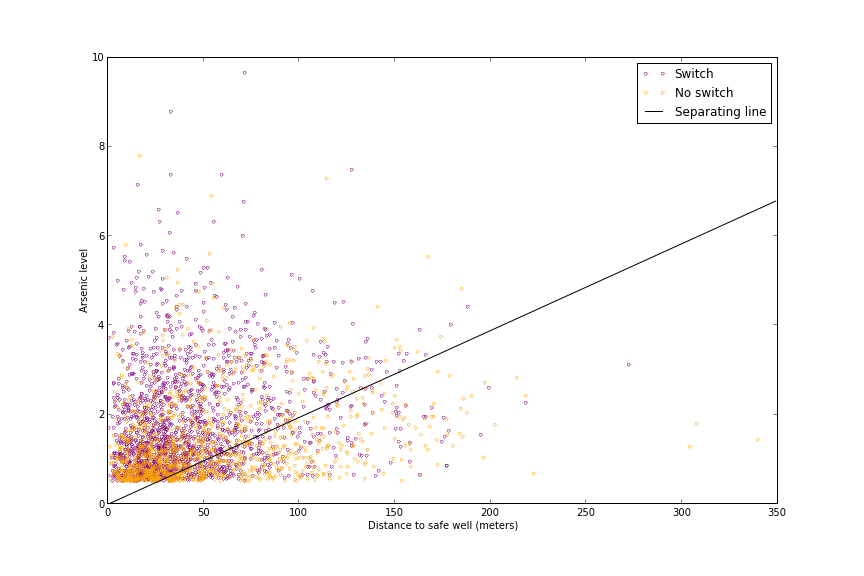
\includegraphics[height=6cm]{wells_2.png}
Model 3: Etkilesim eklemek

Arsenik seviyesi ve uzaklik degiskenlerinin modele ayri ayri yaptigi
etkiler yaninda, beraber olarak ta bazi etkiler yapacagini
dusunebiliriz.  100 metrelik mesafenin degisim kararina olan etkisi
kuyunuzdaki arsenik seviyesiyle baglantili olabilmesi.. Insanlarin
boyle dusunmesini bekleyebiliriz, yani, bu problem baglaminda, tipik
kisi durup ta "once arsenik yokmus gibi dusuneyim, sadece mesafeye
bakayim", sonra "simdi arsenigi dusuneyim, mesafe yokmus gibi
yapayim", ve bunlardan sonra "simdi bu iki ayri karari ust uste
koyayim" seklinde dusunmez.

Patsy ile modele etkilesim eklemenin yolu degiskenler arasinda `:`
operatorunu kullanmak ile olur.

\begin{minted}{python}
model3 = logit('switch ~ I(dist / 100.) + arsenic + I(dist / 100.):arsenic', df).fit()
print model3.summary()
\end{minted}

\begin{verbatim}
Optimization terminated successfully.
         Current function value: 0.650270
         Iterations 5
                           Logit Regression Results                           
==============================================================================
Dep. Variable:                 switch   No. Observations:                 3020
Model:                          Logit   Df Residuals:                     3016
Method:                           MLE   Df Model:                            3
Date:                Tue, 03 Dec 2013   Pseudo R-squ.:                 0.04625
Time:                        10:31:19   Log-Likelihood:                -1963.8
converged:                       True   LL-Null:                       -2059.0
                                        LLR p-value:                 4.830e-41
==========================================================================================
                             coef    std err          z      P>|z|      [95.0% Conf. Int.]
------------------------------------------------------------------------------------------
Intercept                 -0.1479      0.118     -1.258      0.208        -0.378     0.083
I(dist / 100.)            -0.5772      0.209     -2.759      0.006        -0.987    -0.167
arsenic                    0.5560      0.069      8.021      0.000         0.420     0.692
I(dist / 100.):arsenic    -0.1789      0.102     -1.748      0.080        -0.379     0.022
==========================================================================================
\end{verbatim}

Sonuca gore etkilesimin katsayisi negatif ve istatistiki olarak
anlamli (significant) [3]. Bu katsayinin degisim uzerindeki etkisini
nicesel olarak hemen bakar bakmaz anlayamiyor olsak bile, niteliksel
olarak etkisi sezgilerimiz ile uyusuyor. Uzaklik degisimde negatif etkili,
ama bu negatif etki yuksek arsenik seviyesi devreye girince azaliyor.
Diger yandan arsenik seviyesinin degisimde pozitif etkisi var, ama o
etki en yakin kuyu mesafesi arttikca azaliyor. 

Model 4: Egitim seviyesi ve ek bazi etkilesimler, ve degiskenleri ortalamak

Egitim seviyesi kisilerin arsenigin kotu etkilerini anlamasinda
pozitif etki yapmasi beklenir, ve bu sebeple egitim seviyesi degisim
kararina pozitif etki yapmalidir. Elimizdeki veride egitim yil bazinda
kayitlanmis, biz bu veri noktasini olcekleyecegiz (aynen uzakliga
yaptimiz gibi, cunku egitimde 1 senelik degisimin pek bir anlami yok),
bunu icin 4'e bolecegiz. Ayrica bu yeni degiskenin diger degiskenler
ile etkilesimini devreye sokacagiz.

Ek olarak tum degiskenleri ortalayacagiz ki boylece onlari
yorumlamamiz rahatlasacak. Bir kez daha bu isi tamamen Patsy sayesinde
formul icinde halledecegiz, disaridan on hesap yapip formule gecmemiz
gerekmeyecek.

\begin{minted}{python}
model_form = ('switch ~ center(I(dist / 100.)) + center(arsenic) + ' +
              'center(I(educ / 4.)) + ' +
              'center(I(dist / 100.)) : center(arsenic) + ' + 
              'center(I(dist / 100.)) : center(I(educ / 4.)) + ' + 
              'center(arsenic) : center(I(educ / 4.))'
             )
model4 = logit(model_form, df).fit()
print model4.summary()
\end{minted}

\begin{verbatim}
Optimization terminated successfully.
         Current function value: 0.644328
         Iterations 5
                           Logit Regression Results                           
==============================================================================
Dep. Variable:                 switch   No. Observations:                 3020
Model:                          Logit   Df Residuals:                     3013
Method:                           MLE   Df Model:                            6
Date:                Tue, 03 Dec 2013   Pseudo R-squ.:                 0.05497
Time:                        10:31:49   Log-Likelihood:                -1945.9
converged:                       True   LL-Null:                       -2059.0
                                        LLR p-value:                 4.588e-46
===============================================================================================================
                                                  coef    std err          z      P>|z|      [95.0% Conf. Int.]
---------------------------------------------------------------------------------------------------------------
Intercept                                       0.3563      0.040      8.844      0.000         0.277     0.435
center(I(dist / 100.))                         -0.9029      0.107     -8.414      0.000        -1.113    -0.693
center(arsenic)                                 0.4950      0.043     11.497      0.000         0.411     0.579
center(I(educ / 4.))                            0.1850      0.039      4.720      0.000         0.108     0.262
center(I(dist / 100.)):center(arsenic)         -0.1177      0.104     -1.137      0.256        -0.321     0.085
center(I(dist / 100.)):center(I(educ / 4.))     0.3227      0.107      3.026      0.002         0.114     0.532
center(arsenic):center(I(educ / 4.))            0.0722      0.044      1.647      0.100        -0.014     0.158
===============================================================================================================
\end{verbatim}

Modelin basarisini irdelemek: Kutulanmis Kalinti grafikleri (Binned Residual plots)

Model kalintisinin (yani model ile gercek veri arasindaki hatalar
-residual-) ile ayri ayri her degisken ile grafikleri,
uzaklik-kalinti, arsenik-kalinti gibi, bizi modelde gayri lineerlik
olup olmadigi hakkinda uyarabilir. Cunku kalintinin Gaussian bir
dagilimda olmasini bekleriz, model hatasi tam anlamiyla bir "gurultu"
halinde olmalidir, ki dogada gurultunun tanimi Gaussian dagilimina
sahip olmaktir. Eger bu grafikte kabaca her yere esit sekilde dagilmis
bir goruntu gormuyorsak, o zaman modelimizde yakalayamadigimiz bir
gayri lineerlik (nonlinearity) vardir, ya da, birbirinden farkli olan
kalinti grafikleri kalintilari dagilimlarinin birbirinden farkli
oldugunun isaretidir (heteroskedasticity). 

Ikili bir modelde kalintilari ham sekilde grafiklemenin pek anlami
yoktur, o sebeple biraz puruzsuzlestirme uygulayacagiz. Altta
degiskenler icin olusturdugumuz kutucuklar (bins) icine kalintilarin
ortalamasini koyacagiz ve bunlari grafikleyecegiz (lowess ya da hareketli
ortalama -moving average- teknigi de burada ise yarayabilirdi). 

\begin{minted}{python}
def bin_residuals(resid, var, bins):
    '''
    Compute average residuals within bins of a variable.
    
    Returns a dataframe indexed by the bins, with the bin midpoint,
    the residual average within the bin, and the confidence interval 
    bounds.
    '''
    resid_df = DataFrame({'var': var, 'resid': resid})
    resid_df['bins'] = qcut(var, bins)
    bin_group = resid_df.groupby('bins')
    bin_df = bin_group['var', 'resid'].mean()
    bin_df['count'] = bin_group['resid'].count()
    bin_df['lower_ci'] = -2 * (bin_group['resid'].std() / 
                               np.sqrt(bin_group['resid'].count()))
    bin_df['upper_ci'] =  2 * (bin_group['resid'].std() / 
                               np.sqrt(bin_df['count']))
    bin_df = bin_df.sort('var')
    return(bin_df)

def plot_binned_residuals(bin_df):
    '''
    Plotted binned residual averages and confidence intervals.
    '''
    plt.plot(bin_df['var'], bin_df['resid'], '.')
    plt.plot(bin_df['var'], bin_df['lower_ci'], '-r')
    plt.plot(bin_df['var'], bin_df['upper_ci'], '-r')
    plt.axhline(0, color = 'gray', lw = .5)
    
arsenic_resids = bin_residuals(model4.resid, df['arsenic'], 40)
dist_resids = bin_residuals(model4.resid, df['dist'], 40)
plt.figure(figsize = (12, 5))
plt.subplot(121)
plt.ylabel('Residual (bin avg.)')
plt.xlabel('Arsenic (bin avg.)')
plot_binned_residuals(arsenic_resids)
plt.subplot(122)
plot_binned_residuals(dist_resids)
plt.ylabel('Residual (bin avg.)')
plt.xlabel('Distance (bin avg.)')
plt.savefig('wells_3.png')
\end{minted}

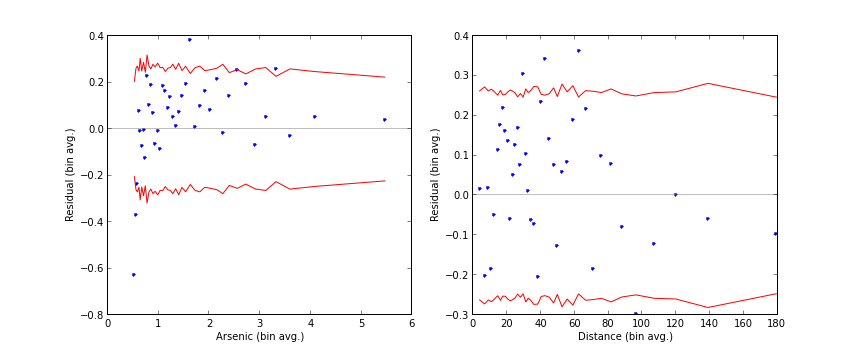
\includegraphics[height=6cm]{wells_3.png}

Ustteki kutulama sirasinda kullanilan <code>qcut</code> islemlerin
icin en altta ek bolumune bakin

Model 5: arsenigi log olceklemek

Kutulanmis artik grafiklerine bakinca arsenik degiskeninde biraz gayri
lineerlik goruyoruz, cunku noktalarin dagilimi cok fazla belli bir
bolgede. Dikkat edelim, model nasil dusuk arsenigi gercekte oldugundan
daha fazla olacagini tahmin etmis (overestimate), ayrica yuksek
arsenigi gercekte oldugundan daha az olacagini tahmin etmis
(underestimate). Bu bize arsenik degiskeni uzerinde belki de log
transformasyonu gibi bir seyler yapmamizin gerektiginin isareti.

Bu degisimi de direk formul icinde yapabiliriz.

\begin{minted}{python}
model_form = ('switch ~ center(I(dist / 100.)) + center(np.log(arsenic)) + ' +
              'center(I(educ / 4.)) + ' +
              'center(I(dist / 100.)) : center(np.log(arsenic)) + ' + 
              'center(I(dist / 100.)) : center(I(educ / 4.)) + ' + 
              'center(np.log(arsenic)) : center(I(educ / 4.))'
             )

model5 = logit(model_form, df).fit()
print model5.summary()
\end{minted}

\begin{verbatim}
Optimization terminated successfully.
         Current function value: 0.639587
         Iterations 5
                           Logit Regression Results                           
==============================================================================
Dep. Variable:                 switch   No. Observations:                 3020
Model:                          Logit   Df Residuals:                     3013
Method:                           MLE   Df Model:                            6
Date:                Tue, 03 Dec 2013   Pseudo R-squ.:                 0.06192
Time:                        10:33:28   Log-Likelihood:                -1931.6
converged:                       True   LL-Null:                       -2059.0
                                        LLR p-value:                 3.517e-52
==================================================================================================================
                                                     coef    std err          z      P>|z|      [95.0% Conf. Int.]
------------------------------------------------------------------------------------------------------------------
Intercept                                          0.3452      0.040      8.528      0.000         0.266     0.425
center(I(dist / 100.))                            -0.9796      0.111     -8.809      0.000        -1.197    -0.762
center(np.log(arsenic))                            0.9036      0.070     12.999      0.000         0.767     1.040
center(I(educ / 4.))                               0.1785      0.039      4.577      0.000         0.102     0.255
center(I(dist / 100.)):center(np.log(arsenic))    -0.1567      0.185     -0.846      0.397        -0.520     0.206
center(I(dist / 100.)):center(I(educ / 4.))        0.3384      0.108      3.141      0.002         0.127     0.550
center(np.log(arsenic)):center(I(educ / 4.))       0.0601      0.070      0.855      0.393        -0.078     0.198
==================================================================================================================
\end{verbatim}

Simdi arsenik icin kutulanmis kalinti grafikleri daha iyi gozukuyor.

\begin{minted}{python}
arsenic_resids = bin_residuals(model5.resid, df['arsenic'], 40)
dist_resids = bin_residuals(model5.resid, df['dist'], 40)
plt.figure(figsize = (12, 5))
plt.subplot(121)
plot_binned_residuals(arsenic_resids)
plt.ylabel('Residual (bin avg.)')
plt.xlabel('Arsenic (bin avg.)')
plt.subplot(122)
plot_binned_residuals(dist_resids)
plt.ylabel('Residual (bin avg.)')
plt.xlabel('Distance (bin avg.)')
plt.savefig('wells_4.png')
\end{minted}

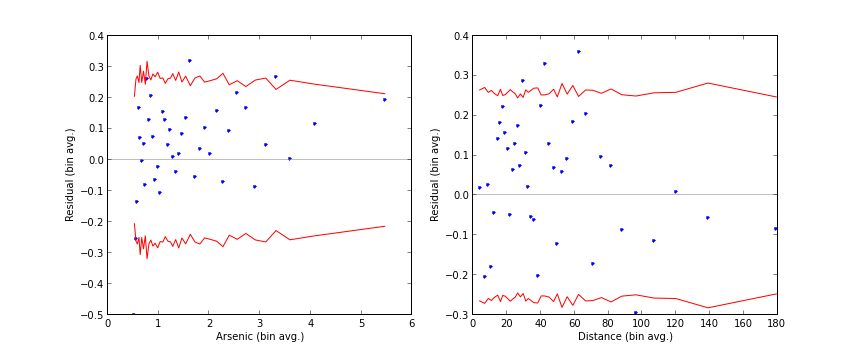
\includegraphics[height=6cm]{wells_4.png}

Model hata oranlari

\verb!pred_table()! cagrisi bize bu modelin "kafa karisikligi matrisini
(confusion matrix)" veriyor [4]. Bu matrisi kullanarak modelimizin hata
oranini hesaplayabiliriz.

Sonra bu sonucu, en fazla verilen cevabi herkesin cevabiymis gibi
farzeden daha basit bir "null modelinin" hata orani ile
karsilastirmaliyiz. Mesela burada kisilerin \%58'i kuyu degistirmis, bu
durumda null modeli "herkes kuyu degistiriyor" diye modeller, ve bu
basit modelin hata payi 42\% olur. Bizim model bu modelden daha iyi
bir sonuc verecek midir? Sonuc altta.

\begin{minted}{python}
print model5.pred_table()
print 'Model Error rate: {0: 3.0%}'.format(
    1 - np.diag(model5.pred_table()).sum() / model5.pred_table().sum())
print 'Null Error Rate: {0: 3.0%}'.format(
    1 - df['switch'].mean())
\end{minted}

\begin{verbatim}
[[  568.   715.]
 [  387.  1350.]]
Model Error rate:  36%
Null Error Rate:  42%
\end{verbatim}

Ek: qcut

Yukaridaki qcut kullanimini ozetlemek gerekirse; arsenik degiskeni
icin mesela dagilim bolgeleri (n-tile) uzerinden bir atama yapacagiz,
once DataFrame yaratalim,

\begin{minted}{python}
resid_df = DataFrame({'var': df['arsenic'], 'resid': model4.resid})
print resid_df[:10]
\end{minted}

\begin{verbatim}
       resid   var
1   0.842596  2.36
2   1.281417  0.71
3  -1.613751  2.07
4   0.996195  1.15
5   1.005102  1.10
6   0.592056  3.90
7   0.941372  2.97
8   0.640139  3.24
9   0.886626  3.28
10  1.130149  2.52
\end{verbatim}

Simdi 40 tane dagilim bolgesi yaratalim

\begin{minted}{python}
print qcut(df['arsenic'], 40)
\end{minted}

\begin{verbatim}
Categorical: arsenic
[(2.327, 2.47], (0.68, 0.71], (1.953, 2.07], (1.1, 1.15], (1.0513, 1.1], (3.791, 4.475], (2.81, 2.98], (3.21, 3.42], (3.21, 3.42], (2.47, 2.61], (2.98, 3.21], (2.98, 3.21], (2.81, 2.98], (2.98, 3.21], (1.66, 1.76], (1.76, 1.858], (1.42, 1.49], (1.42, 1.49], (2.327, 2.47], (2.81, 2.98], (1.76, 1.858], (2.47, 2.61], (2.2, 2.327], (2.327, 2.47], (1.57, 1.66], (2.327, 2.47], (3.42, 3.791], (2.07, 2.2], (0.9, 0.95], (3.21, 3.42], (1.42, 1.49], (0.82, 0.86], (1.36, 1.42], (2.61, 2.81], (0.78, 0.82], (1.42, 1.49], (1.858, 1.953], (2.61, 2.81], (2.47, 2.61], (3.791, 4.475], (2.61, 2.81], (2.81, 2.98], (0.82, 0.86], (3.42, 3.791], (2.81, 2.98], (0.75, 0.78], (2.47, 2.61], (2.47, 2.61], (3.791, 4.475], (1.49, 1.57], (1.76, 1.858], [0.51, 0.53], (0.62, 0.64], (1.0065, 1.0513], (0.71, 0.75], (1.76, 1.858], (2.61, 2.81], (4.475, 9.65], (2.98, 3.21], (4.475, 9.65], (2.61, 2.81], (0.56, 0.59], (4.475, 9.65], (3.791, 4.475], (0.86, 0.9], (0.95, 1.0065], (0.9, 0.95], (3.42, 3.791], (4.475, 9.65], (4.475, 9.65], (1.953, 2.07], (2.81, 2.98], (0.78, 0.82], (2.81, 2.98], (2.07, 2.2], (3.791, 4.475], (1.858, 1.953], (1.57, 1.66], (4.475, 9.65], (1.49, 1.57], (1.858, 1.953], (1.57, 1.66], (0.64, 0.68], (1.36, 1.42], (1.15, 1.2], (0.75, 0.78], (0.75, 0.78], (1.42, 1.49], (0.75, 0.78], (0.75, 0.78], (0.71, 0.75], (1.858, 1.953], (0.71, 0.75], (0.86, 0.9], (1.0065, 1.0513], (1.2, 1.25], (1.42, 1.49], (0.62, 0.64], (0.78, 0.82], (1.858, 1.953], (0.53, 0.56], (1.3, 1.36], [0.51, 0.53], (1.15, 1.2], (1.15, 1.2], (1.25, 1.3], (0.86, 0.9], (2.98, 3.21], (2.07, 2.2], (0.75, 0.78], (0.53, 0.56], (0.59, 0.62], (1.0065, 1.0513], (0.75, 0.78], (1.0065, 1.0513], (0.64, 0.68], (2.2, 2.327], (1.57, 1.66], (0.78, 0.82], (1.42, 1.49], (0.95, 1.0065], (0.86, 0.9], (1.36, 1.42], (0.82, 0.86], (0.56, 0.59], (1.42, 1.49], (1.1, 1.15], (2.327, 2.47], (3.791, 4.475], (3.42, 3.791], (3.42, 3.791], (2.81, 2.98], (2.98, 3.21], (3.42, 3.791], (3.791, 4.475], (3.791, 4.475], (3.42, 3.791], (3.791, 4.475], (3.791, 4.475], (3.791, 4.475], (3.21, 3.42], (1.953, 2.07], (1.42, 1.49], (2.2, 2.327], (1.36, 1.42], (2.327, 2.47], (1.49, 1.57], (1.42, 1.49], (1.49, 1.57], (1.3, 1.36], (0.53, 0.56], (1.15, 1.2], (1.0065, 1.0513], (1.1, 1.15], [0.51, 0.53], (0.53, 0.56], (0.59, 0.62], (2.07, 2.2], (0.59, 0.62], (0.95, 1.0065], (0.9, 0.95], (0.9, 0.95], (1.0065, 1.0513], (1.2, 1.25], (1.36, 1.42], (1.3, 1.36], (0.82, 0.86], (2.61, 2.81], (1.76, 1.858], (2.47, 2.61], (1.25, 1.3], (0.68, 0.71], (0.59, 0.62], (0.86, 0.9], (0.71, 0.75], (0.78, 0.82], (1.76, 1.858], (1.2, 1.25], (1.1, 1.15], (0.68, 0.71], (2.07, 2.2], (1.66, 1.76], (1.76, 1.858], (1.25, 1.3], (2.47, 2.61], (2.81, 2.98], (0.59, 0.62], (2.98, 3.21], (2.47, 2.61], (1.953, 2.07], (1.15, 1.2], (0.86, 0.9], [0.51, 0.53], (2.47, 2.61], (1.2, 1.25], (1.1, 1.15], (1.1, 1.15], [0.51, 0.53], (0.86, 0.9], (3.42, 3.791], (0.53, 0.56], (1.3, 1.36], (1.66, 1.76], (1.858, 1.953], (2.327, 2.47], (2.327, 2.47], (2.327, 2.47], (1.42, 1.49], (1.953, 2.07], (1.3, 1.36], (1.66, 1.76], (1.76, 1.858], (1.66, 1.76], (1.76, 1.858], (2.61, 2.81], (0.71, 0.75], (0.68, 0.71], (0.56, 0.59], [0.51, 0.53], (0.59, 0.62], (3.21, 3.42], [0.51, 0.53], (1.25, 1.3], (0.59, 0.62], (0.56, 0.59], (0.64, 0.68], (0.71, 0.75], (0.68, 0.71], (0.82, 0.86], [0.51, 0.53], (0.56, 0.59], (0.53, 0.56], (1.25, 1.3], [0.51, 0.53], (0.82, 0.86], (0.56, 0.59], [0.51, 0.53], (0.64, 0.68], (3.42, 3.791], (2.61, 2.81], (0.75, 0.78], (0.71, 0.75], (0.75, 0.78], (1.57, 1.66], (0.78, 0.82], (0.53, 0.56], (0.86, 0.9], [0.51, 0.53], (2.47, 2.61], (1.25, 1.3], (0.95, 1.0065], (1.42, 1.49], (1.0065, 1.0513], (0.9, 0.95], (0.78, 0.82], (0.64, 0.68], (0.82, 0.86], (0.9, 0.95], (1.36, 1.42], (0.71, 0.75], (1.42, 1.49], (1.15, 1.2], (1.15, 1.2], (0.82, 0.86], (1.2, 1.25], (2.98, 3.21], (3.42, 3.791], (1.953, 2.07], (1.66, 1.76], (1.66, 1.76], (2.61, 2.81], (1.25, 1.3], (1.42, 1.49], (0.95, 1.0065], [0.51, 0.53], (0.64, 0.68], (0.68, 0.71], [0.51, 0.53], (1.0065, 1.0513], (1.953, 2.07], (0.75, 0.78], (1.15, 1.2], (0.59, 0.62], (1.3, 1.36], (1.76, 1.858], (0.53, 0.56], (0.75, 0.78], (0.64, 0.68], (1.0513, 1.1], (0.78, 0.82], (2.2, 2.327], (2.81, 2.98], (0.62, 0.64], (1.25, 1.3], (1.49, 1.57], (1.76, 1.858], (1.2, 1.25], (0.9, 0.95], (0.53, 0.56], (0.78, 0.82], (0.59, 0.62], (0.68, 0.71], (0.78, 0.82], (0.64, 0.68], (0.64, 0.68], (1.25, 1.3], (0.9, 0.95], (1.2, 1.25], (1.15, 1.2], (0.75, 0.78], (1.15, 1.2], (0.86, 0.9], [0.51, 0.53], [0.51, 0.53], (0.62, 0.64], (1.953, 2.07], (0.56, 0.59], (1.42, 1.49], (1.76, 1.858], (1.36, 1.42], (1.49, 1.57], (1.858, 1.953], (1.57, 1.66], (0.68, 0.71], [0.51, 0.53], (2.47, 2.61], (0.62, 0.64], (1.0513, 1.1], (0.68, 0.71], (1.1, 1.15], [0.51, 0.53], (0.56, 0.59], (1.3, 1.36], (1.42, 1.49], (0.82, 0.86], (0.62, 0.64], (1.42, 1.49], (1.49, 1.57], (1.25, 1.3], (2.07, 2.2], (1.66, 1.76], (1.858, 1.953], (2.07, 2.2], (1.57, 1.66], (1.57, 1.66], (0.78, 0.82], (1.858, 1.953], (1.858, 1.953], (1.858, 1.953], (3.791, 4.475], (3.791, 4.475], (1.49, 1.57], (2.47, 2.61], (3.21, 3.42], (2.2, 2.327], (2.81, 2.98], (1.953, 2.07], (3.791, 4.475], (2.81, 2.98], (1.36, 1.42], (1.953, 2.07], (1.42, 1.49], (1.49, 1.57], (3.21, 3.42], (3.791, 4.475], (2.47, 2.61], (0.75, 0.78], (2.2, 2.327], (1.42, 1.49], (1.66, 1.76], (1.953, 2.07], (2.47, 2.61], (3.791, 4.475], (3.791, 4.475], (2.98, 3.21], (3.21, 3.42], (3.42, 3.791], (1.36, 1.42], (1.858, 1.953], (2.61, 2.81], (3.42, 3.791], (1.953, 2.07], (2.07, 2.2], (2.61, 2.81], (3.21, 3.42], (3.21, 3.42], (1.49, 1.57], (2.47, 2.61], (1.953, 2.07], (2.81, 2.98], (2.47, 2.61], (3.42, 3.791], (4.475, 9.65], (1.57, 1.66], (2.2, 2.327], (2.327, 2.47], (2.327, 2.47], (1.2, 1.25], (3.791, 4.475], (4.475, 9.65], (1.858, 1.953], (2.327, 2.47], (2.07, 2.2], (4.475, 9.65], (3.42, 3.791], (3.42, 3.791], (2.98, 3.21], (2.61, 2.81], (2.327, 2.47], (2.98, 3.21], (2.47, 2.61], (3.21, 3.42], (2.2, 2.327], (3.42, 3.791], (1.0065, 1.0513], (3.21, 3.42], (1.57, 1.66], (1.15, 1.2], (1.0065, 1.0513], (0.64, 0.68], (2.98, 3.21], (2.327, 2.47], (2.2, 2.327], (1.57, 1.66], (3.791, 4.475], (3.21, 3.42], (2.98, 3.21], (3.21, 3.42], (1.57, 1.66], (3.21, 3.42], (2.98, 3.21], (3.42, 3.791], (3.791, 4.475], (2.81, 2.98], (0.9, 0.95], (2.47, 2.61], (3.21, 3.42], (3.21, 3.42], (3.21, 3.42], (3.21, 3.42], (3.21, 3.42], (2.81, 2.98], (1.42, 1.49], (3.791, 4.475], (1.858, 1.953], (2.98, 3.21], (2.98, 3.21], (2.61, 2.81], (3.21, 3.42], (1.858, 1.953], (3.42, 3.791], (2.47, 2.61], (2.81, 2.98], (2.81, 2.98], (2.2, 2.327], (2.98, 3.21], (3.42, 3.791], (2.98, 3.21], (2.81, 2.98], (1.858, 1.953], (1.76, 1.858], (2.07, 2.2], (1.66, 1.76], (3.791, 4.475], (3.42, 3.791], (3.791, 4.475], (1.36, 1.42], (4.475, 9.65], (2.07, 2.2], (2.47, 2.61], (1.76, 1.858], (1.2, 1.25], (1.36, 1.42], (1.49, 1.57], [0.51, 0.53], (0.86, 0.9], (1.953, 2.07], (0.59, 0.62], (0.53, 0.56], [0.51, 0.53], (0.75, 0.78], (0.64, 0.68], (0.64, 0.68], (0.62, 0.64], (0.56, 0.59], (0.75, 0.78], (0.71, 0.75], (0.86, 0.9], (0.59, 0.62], (2.2, 2.327], (1.2, 1.25], (1.2, 1.25], (2.327, 2.47], (1.15, 1.2], (2.327, 2.47], (2.81, 2.98], (3.21, 3.42], (1.49, 1.57], (0.53, 0.56], (0.82, 0.86], (2.2, 2.327], (1.66, 1.76], (2.2, 2.327], (0.82, 0.86], [0.51, 0.53], (1.57, 1.66], (1.953, 2.07], (1.66, 1.76], (0.53, 0.56], (1.42, 1.49], (0.71, 0.75], (0.59, 0.62], (0.56, 0.59], (0.82, 0.86], (3.42, 3.791], (3.42, 3.791], (0.9, 0.95], (0.56, 0.59], (1.2, 1.25], (1.2, 1.25], (0.56, 0.59], (1.66, 1.76], (1.15, 1.2], (1.0513, 1.1], (0.71, 0.75], (1.0065, 1.0513], (1.0513, 1.1], (1.0065, 1.0513], (0.56, 0.59], [0.51, 0.53], (0.62, 0.64], (2.327, 2.47], (1.49, 1.57], (2.61, 2.81], (3.791, 4.475], (0.9, 0.95], (0.62, 0.64], (0.53, 0.56], (0.53, 0.56], (3.42, 3.791], (0.53, 0.56], (0.56, 0.59], (0.56, 0.59], [0.51, 0.53], (0.62, 0.64], (0.53, 0.56], (0.68, 0.71], (0.71, 0.75], (0.68, 0.71], (0.78, 0.82], (0.9, 0.95], [0.51, 0.53], (0.56, 0.59], (0.68, 0.71], [0.51, 0.53], (0.78, 0.82], (0.68, 0.71], (0.95, 1.0065], [0.51, 0.53], (0.71, 0.75], (0.64, 0.68], (0.78, 0.82], (0.68, 0.71], (1.0065, 1.0513], (2.61, 2.81], (1.2, 1.25], (0.59, 0.62], (0.68, 0.71], (2.61, 2.81], (1.49, 1.57], (1.76, 1.858], [0.51, 0.53], (0.9, 0.95], (0.59, 0.62], (1.1, 1.15], (3.21, 3.42], (1.15, 1.2], (0.64, 0.68], [0.51, 0.53], (0.64, 0.68], [0.51, 0.53], (1.2, 1.25], (0.56, 0.59], (0.95, 1.0065], (0.64, 0.68], [0.51, 0.53], (1.1, 1.15], (0.64, 0.68], [0.51, 0.53], (0.62, 0.64], (1.953, 2.07], (0.71, 0.75], (0.9, 0.95], (0.78, 0.82], (0.64, 0.68], (0.82, 0.86], (0.78, 0.82], (0.56, 0.59], (0.64, 0.68], [0.51, 0.53], (0.56, 0.59], (0.53, 0.56], (0.9, 0.95], (0.59, 0.62], (0.71, 0.75], (0.68, 0.71], (0.56, 0.59], (1.0065, 1.0513], (0.64, 0.68], (0.56, 0.59], (0.82, 0.86], (0.71, 0.75], (0.75, 0.78], [0.51, 0.53], (0.53, 0.56], (0.59, 0.62], (1.0513, 1.1], (1.0513, 1.1], (0.64, 0.68], (1.2, 1.25], (1.15, 1.2], (1.2, 1.25], (0.75, 0.78], (0.86, 0.9], (1.1, 1.15], (0.56, 0.59], (2.81, 2.98], (2.61, 2.81], (0.95, 1.0065], (2.327, 2.47], (2.327, 2.47], (1.3, 1.36], (2.98, 3.21], (1.36, 1.42], (2.98, 3.21], (2.81, 2.98], (3.21, 3.42], (1.858, 1.953], (2.81, 2.98], (2.2, 2.327], (1.953, 2.07], (3.42, 3.791], (4.475, 9.65], (3.791, 4.475], (1.57, 1.66], (1.953, 2.07], (2.81, 2.98], (3.791, 4.475], (3.21, 3.42], (2.47, 2.61], (2.61, 2.81], (1.49, 1.57], (2.47, 2.61], (0.86, 0.9], (2.327, 2.47], (2.61, 2.81], (3.791, 4.475], (1.25, 1.3], (3.791, 4.475], (2.2, 2.327], (2.2, 2.327], (1.57, 1.66], (1.0513, 1.1], (1.76, 1.858], (0.59, 0.62], (0.62, 0.64], (2.07, 2.2], (1.953, 2.07], (2.81, 2.98], (2.07, 2.2], (1.66, 1.76], (2.327, 2.47], (2.47, 2.61], (1.858, 1.953], (1.858, 1.953], (0.82, 0.86], (1.66, 1.76], (1.76, 1.858], (2.07, 2.2], (2.47, 2.61], (1.66, 1.76], (3.21, 3.42], (1.76, 1.858], (2.07, 2.2], (1.3, 1.36], (1.858, 1.953], (3.791, 4.475], (1.36, 1.42], (0.59, 0.62], (1.57, 1.66], (0.82, 0.86], (0.9, 0.95], [0.51, 0.53], (1.953, 2.07], (0.9, 0.95], (0.59, 0.62], (0.71, 0.75], (0.62, 0.64], (3.42, 3.791], (1.15, 1.2], (1.3, 1.36], (0.86, 0.9], (2.327, 2.47], (2.2, 2.327], (1.2, 1.25], (1.0513, 1.1], (2.07, 2.2], (1.76, 1.858], (1.49, 1.57], (1.57, 1.66], (0.82, 0.86], (1.42, 1.49], (1.57, 1.66], (0.64, 0.68], (1.66, 1.76], (1.57, 1.66], (0.68, 0.71], (1.3, 1.36], (1.1, 1.15], (1.0065, 1.0513], (2.2, 2.327], (1.36, 1.42], (0.59, 0.62], (2.98, 3.21], (1.36, 1.42], [0.51, 0.53], (1.0513, 1.1], [0.51, 0.53], (0.86, 0.9], (1.2, 1.25], (0.9, 0.95], (0.64, 0.68], (2.07, 2.2], (2.327, 2.47], (1.66, 1.76], (2.81, 2.98], (2.61, 2.81], (1.49, 1.57], (1.25, 1.3], (1.3, 1.36], (1.953, 2.07], (2.2, 2.327], (2.47, 2.61], (3.21, 3.42], (2.61, 2.81], (2.47, 2.61], (2.327, 2.47], (3.42, 3.791], (2.98, 3.21], (2.47, 2.61], (2.07, 2.2], (4.475, 9.65], (3.21, 3.42], (3.21, 3.42], (2.81, 2.98], (1.0513, 1.1], (2.61, 2.81], (1.25, 1.3], (3.21, 3.42], (0.82, 0.86], (2.47, 2.61], (0.53, 0.56], (1.57, 1.66], (2.81, 2.98], (1.1, 1.15], (1.0513, 1.1], (2.81, 2.98], (0.64, 0.68], (1.0513, 1.1], (1.66, 1.76], (2.81, 2.98], (2.47, 2.61], (2.07, 2.2], (1.953, 2.07], (1.76, 1.858], (1.858, 1.953], (1.3, 1.36], (3.21, 3.42], (1.36, 1.42], (1.49, 1.57], (0.82, 0.86], (0.95, 1.0065], (0.86, 0.9], (1.3, 1.36], (1.57, 1.66], (2.98, 3.21], (0.82, 0.86], (1.25, 1.3], (2.47, 2.61], (1.49, 1.57], (1.66, 1.76], (1.1, 1.15], (3.21, 3.42], (2.327, 2.47], (1.49, 1.57], (2.2, 2.327], (2.81, 2.98], (1.57, 1.66], (2.47, 2.61], (1.0513, 1.1], (0.78, 0.82], (2.327, 2.47], (1.2, 1.25], (1.76, 1.858], (2.47, 2.61], (2.47, 2.61], (2.98, 3.21], (2.81, 2.98], (2.61, 2.81], (3.42, 3.791], (0.9, 0.95], (1.15, 1.2], (3.791, 4.475], (2.07, 2.2], (2.98, 3.21], (3.42, 3.791], (1.76, 1.858], (4.475, 9.65], (3.791, 4.475], (4.475, 9.65], (3.791, 4.475], (4.475, 9.65], (4.475, 9.65], (4.475, 9.65], (1.49, 1.57], (2.61, 2.81], (3.791, 4.475], (3.42, 3.791], (2.61, 2.81], (2.98, 3.21], (2.98, 3.21], (1.25, 1.3], (4.475, 9.65], (4.475, 9.65], (4.475, 9.65], (3.791, 4.475], (1.858, 1.953], (0.82, 0.86], (3.791, 4.475], (3.791, 4.475], (3.42, 3.791], (3.21, 3.42], (2.98, 3.21], (3.791, 4.475], (3.42, 3.791], (3.21, 3.42], (2.47, 2.61], (1.25, 1.3], (1.953, 2.07], (3.21, 3.42], (3.42, 3.791], (3.791, 4.475], (3.21, 3.42], (4.475, 9.65], (4.475, 9.65], (1.3, 1.36], (0.68, 0.71], (1.15, 1.2], (0.56, 0.59], (1.42, 1.49], (0.53, 0.56], (0.95, 1.0065], (1.42, 1.49], (1.42, 1.49], (1.57, 1.66], (1.66, 1.76], (1.3, 1.36], (0.95, 1.0065], (0.71, 0.75], (1.0513, 1.1], (1.0513, 1.1], (0.59, 0.62], (0.9, 0.95], (1.25, 1.3], (0.68, 0.71], (1.25, 1.3], (0.62, 0.64], (0.62, 0.64], (0.71, 0.75], (0.53, 0.56], (0.59, 0.62], (0.82, 0.86], (1.0065, 1.0513], (1.2, 1.25], (0.64, 0.68], (0.64, 0.68], (0.56, 0.59], (0.53, 0.56], (2.327, 2.47], (1.3, 1.36], (0.86, 0.9], (0.68, 0.71], (0.64, 0.68], (1.42, 1.49], (0.86, 0.9], (0.82, 0.86], (0.78, 0.82], (0.68, 0.71], (0.59, 0.62], (1.0065, 1.0513], (1.49, 1.57], (1.15, 1.2], (1.49, 1.57], (1.36, 1.42], (0.62, 0.64], (0.59, 0.62], (0.78, 0.82], (1.15, 1.2], (0.9, 0.95], (1.0513, 1.1], (1.42, 1.49], (1.57, 1.66], (1.953, 2.07], (0.53, 0.56], (0.71, 0.75], (0.68, 0.71], (1.36, 1.42], (0.82, 0.86], (1.3, 1.36], (1.858, 1.953], (1.49, 1.57], (1.858, 1.953], (4.475, 9.65], (2.98, 3.21], (4.475, 9.65], (2.327, 2.47], (0.86, 0.9], (0.53, 0.56], (0.78, 0.82], (0.71, 0.75], (3.791, 4.475], (1.42, 1.49], (2.61, 2.81], (0.71, 0.75], (0.62, 0.64], (0.82, 0.86], (1.1, 1.15], (1.15, 1.2], (0.9, 0.95], (1.2, 1.25], (1.0513, 1.1], (1.66, 1.76], (1.0513, 1.1], (0.95, 1.0065], (1.2, 1.25], (1.57, 1.66], (1.1, 1.15], (1.1, 1.15], (1.2, 1.25], (1.57, 1.66], (1.66, 1.76], (1.0513, 1.1], (1.0513, 1.1], (2.2, 2.327], (1.42, 1.49], (1.3, 1.36], (3.42, 3.791], (1.15, 1.2], (0.53, 0.56], (1.0065, 1.0513], (1.49, 1.57], (1.57, 1.66], (0.75, 0.78], (0.64, 0.68], (1.1, 1.15], (0.71, 0.75], (1.57, 1.66], (2.2, 2.327], (0.59, 0.62], (0.64, 0.68], (0.64, 0.68], [0.51, 0.53], (0.64, 0.68], (3.21, 3.42], (2.81, 2.98], (1.3, 1.36], (1.858, 1.953], (1.36, 1.42], (1.36, 1.42], (2.327, 2.47], (0.78, 0.82], (0.59, 0.62], (2.81, 2.98], (1.1, 1.15], (1.49, 1.57], (1.15, 1.2], (2.327, 2.47], (2.47, 2.61], (0.62, 0.64], (1.858, 1.953], (1.76, 1.858], (1.25, 1.3], (0.75, 0.78], (1.858, 1.953], (1.1, 1.15], (0.71, 0.75], (1.15, 1.2], (0.56, 0.59], (0.78, 0.82], (1.2, 1.25], (0.95, 1.0065], (0.71, 0.75], (0.78, 0.82], (0.71, 0.75], (1.0065, 1.0513], [0.51, 0.53], (0.53, 0.56], (0.82, 0.86], [0.51, 0.53], (0.71, 0.75], (0.71, 0.75], (0.64, 0.68], (1.0065, 1.0513], (1.42, 1.49], (1.0513, 1.1], (2.07, 2.2], (1.49, 1.57], (1.76, 1.858], (1.76, 1.858], (2.61, 2.81], (1.858, 1.953], (1.66, 1.76], (2.327, 2.47], [0.51, 0.53], (0.95, 1.0065], (0.9, 0.95], (0.9, 0.95], (1.49, 1.57], (1.42, 1.49], (1.49, 1.57], (1.42, 1.49], (1.0513, 1.1], (1.0065, 1.0513], (0.64, 0.68], (0.56, 0.59], (0.64, 0.68], (0.53, 0.56], (0.68, 0.71], (0.82, 0.86], (1.1, 1.15], (0.62, 0.64], (1.2, 1.25], (0.95, 1.0065], (1.0065, 1.0513], (0.9, 0.95], (2.07, 2.2], (0.9, 0.95], [0.51, 0.53], (0.95, 1.0065], (0.71, 0.75], (0.59, 0.62], (1.42, 1.49], (2.327, 2.47], (0.71, 0.75], (1.0065, 1.0513], (1.25, 1.3], (1.15, 1.2], (1.42, 1.49], (1.3, 1.36], (1.953, 2.07], (1.1, 1.15], (1.0513, 1.1], (1.36, 1.42], (1.953, 2.07], (2.2, 2.327], (1.66, 1.76], (1.42, 1.49], (1.2, 1.25], (1.49, 1.57], (0.71, 0.75], (1.15, 1.2], (1.36, 1.42], (0.95, 1.0065], (1.1, 1.15], (0.71, 0.75], (0.9, 0.95], (1.49, 1.57], (1.3, 1.36], (1.36, 1.42], (1.42, 1.49], (0.71, 0.75], (0.95, 1.0065], (0.71, 0.75], (1.858, 1.953], (1.66, 1.76], (1.858, 1.953], (0.53, 0.56], [0.51, 0.53], (1.25, 1.3], (0.75, 0.78], [0.51, 0.53], (0.68, 0.71], (0.59, 0.62], (0.68, 0.71], (0.95, 1.0065], (0.9, 0.95], (1.2, 1.25], (0.9, 0.95], (1.0065, 1.0513], (0.82, 0.86], (0.78, 0.82], (0.71, 0.75], (0.59, 0.62], (0.71, 0.75], (1.1, 1.15], (0.68, 0.71], (1.0065, 1.0513], (0.59, 0.62], (0.56, 0.59], [0.51, 0.53], [0.51, 0.53], [0.51, 0.53], (0.64, 0.68], (0.64, 0.68], (3.42, 3.791], (1.1, 1.15], (1.3, 1.36], (0.95, 1.0065], (1.76, 1.858], (0.71, 0.75], (0.64, 0.68], (0.62, 0.64], (1.15, 1.2], (1.0065, 1.0513], (1.42, 1.49], (0.78, 0.82], (1.2, 1.25], (0.95, 1.0065], [0.51, 0.53], (0.68, 0.71], (1.76, 1.858], (1.3, 1.36], (0.53, 0.56], (1.2, 1.25], (1.42, 1.49], (1.57, 1.66], (0.86, 0.9], (0.53, 0.56], (1.858, 1.953], (0.9, 0.95], (1.3, 1.36], (1.42, 1.49], (0.95, 1.0065], (0.64, 0.68], (1.42, 1.49], (0.68, 0.71], (1.0065, 1.0513], (1.0065, 1.0513], (0.86, 0.9], (2.98, 3.21], (4.475, 9.65], (1.0513, 1.1], (1.36, 1.42], (1.36, 1.42], (1.25, 1.3], (0.9, 0.95], (0.9, 0.95], (1.0065, 1.0513], (1.49, 1.57], (0.9, 0.95], (1.57, 1.66], (1.42, 1.49], (0.82, 0.86], (0.68, 0.71], (0.95, 1.0065], (0.71, 0.75], (1.25, 1.3], (0.86, 0.9], (0.56, 0.59], (0.71, 0.75], (1.76, 1.858], (1.76, 1.858], (1.57, 1.66], (0.86, 0.9], (1.2, 1.25], (1.66, 1.76], (0.86, 0.9], (0.75, 0.78], (1.953, 2.07], (1.66, 1.76], (1.76, 1.858], (1.66, 1.76], (2.2, 2.327], (1.25, 1.3], (2.81, 2.98], (1.66, 1.76], (2.2, 2.327], (2.47, 2.61], (1.66, 1.76], (0.68, 0.71], (1.42, 1.49], (1.15, 1.2], (1.2, 1.25], (1.3, 1.36], (1.1, 1.15], (0.86, 0.9], (1.57, 1.66], (1.36, 1.42], (1.0065, 1.0513], (0.59, 0.62], (1.1, 1.15], (1.66, 1.76], (2.327, 2.47], (1.49, 1.57], (1.25, 1.3], (1.36, 1.42], (1.15, 1.2], (1.1, 1.15], (2.07, 2.2], (1.66, 1.76], (1.0513, 1.1], (1.15, 1.2], (1.3, 1.36], (1.953, 2.07], (2.81, 2.98], (1.2, 1.25], (2.81, 2.98], (2.61, 2.81], (0.75, 0.78], (1.953, 2.07], (2.2, 2.327], (1.36, 1.42], (0.64, 0.68], (0.59, 0.62], (1.25, 1.3], (1.49, 1.57], (0.71, 0.75], (0.78, 0.82], (0.62, 0.64], (0.64, 0.68], (1.2, 1.25], (1.0513, 1.1], (0.64, 0.68], (1.1, 1.15], (2.07, 2.2], (1.0065, 1.0513], (0.53, 0.56], (0.62, 0.64], (0.64, 0.68], (1.1, 1.15], (1.36, 1.42], (0.82, 0.86], (0.78, 0.82], (1.25, 1.3], (1.953, 2.07], (0.9, 0.95], (0.86, 0.9], (3.791, 4.475], (1.0065, 1.0513], (1.76, 1.858], (3.791, 4.475], (1.66, 1.76], (1.2, 1.25], (0.71, 0.75], (0.71, 0.75], (1.15, 1.2], (1.953, 2.07], (1.3, 1.36], (1.15, 1.2], (0.62, 0.64], (1.1, 1.15], (2.2, 2.327], (2.2, 2.327], (1.3, 1.36], (0.62, 0.64], (1.953, 2.07], (2.81, 2.98], (2.07, 2.2], (1.858, 1.953], (3.42, 3.791], (3.21, 3.42], (0.86, 0.9], (0.59, 0.62], (2.327, 2.47], (1.66, 1.76], (2.81, 2.98], (2.81, 2.98], (1.66, 1.76], (1.76, 1.858], (2.327, 2.47], [0.51, 0.53], (2.47, 2.61], (1.858, 1.953], (2.07, 2.2], (1.2, 1.25], (2.98, 3.21], (1.36, 1.42], (2.327, 2.47], (1.66, 1.76], (2.81, 2.98], (1.76, 1.858], (2.81, 2.98], (2.98, 3.21], (2.61, 2.81], (1.858, 1.953], (1.0513, 1.1], (4.475, 9.65], (3.791, 4.475], (2.2, 2.327], (1.57, 1.66], (2.327, 2.47], (2.2, 2.327], (1.76, 1.858], (2.2, 2.327], (2.98, 3.21], (0.56, 0.59], (1.76, 1.858], (2.81, 2.98], (3.42, 3.791], (1.57, 1.66], (2.2, 2.327], (2.07, 2.2], (1.36, 1.42], (1.2, 1.25], (2.47, 2.61], (1.66, 1.76], (2.98, 3.21], (1.0513, 1.1], (2.47, 2.61], (0.95, 1.0065], (1.953, 2.07], (1.42, 1.49], (1.42, 1.49], (1.3, 1.36], [0.51, 0.53], (0.86, 0.9], (0.9, 0.95], (0.53, 0.56], [0.51, 0.53], (0.82, 0.86], (1.3, 1.36], (1.15, 1.2], (0.9, 0.95], (2.98, 3.21], (2.98, 3.21], (2.98, 3.21], (0.56, 0.59], (1.57, 1.66], (1.42, 1.49], (0.68, 0.71], [0.51, 0.53], (0.62, 0.64], [0.51, 0.53], (0.59, 0.62], (0.68, 0.71], (0.9, 0.95], (0.64, 0.68], (1.2, 1.25], (0.9, 0.95], (1.66, 1.76], (1.2, 1.25], (3.791, 4.475], (1.953, 2.07], (3.791, 4.475], (3.42, 3.791], (2.47, 2.61], (4.475, 9.65], (2.2, 2.327], (2.98, 3.21], (1.66, 1.76], (2.327, 2.47], (1.49, 1.57], (0.82, 0.86], (1.1, 1.15], (0.68, 0.71], (1.3, 1.36], (0.9, 0.95], (0.68, 0.71], (1.15, 1.2], (0.71, 0.75], (0.86, 0.9], (0.95, 1.0065], (1.953, 2.07], (1.2, 1.25], (0.75, 0.78], (0.64, 0.68], (1.2, 1.25], (1.42, 1.49], (1.0065, 1.0513], (1.49, 1.57], (1.49, 1.57], (1.2, 1.25], (0.53, 0.56], (1.2, 1.25], (0.59, 0.62], (1.0065, 1.0513], (0.9, 0.95], (0.56, 0.59], (3.42, 3.791], (0.68, 0.71], (0.78, 0.82], (0.56, 0.59], (1.42, 1.49], (0.9, 0.95], (1.15, 1.2], (1.25, 1.3], (1.3, 1.36], (1.0065, 1.0513], (1.0513, 1.1], (0.56, 0.59], (0.68, 0.71], (0.59, 0.62], (0.64, 0.68], (0.62, 0.64], (0.82, 0.86], (0.62, 0.64], (0.59, 0.62], (0.82, 0.86], (0.59, 0.62], [0.51, 0.53], (2.47, 2.61], [0.51, 0.53], (1.1, 1.15], (1.0065, 1.0513], (0.82, 0.86], (1.0513, 1.1], (3.42, 3.791], (0.53, 0.56], (1.57, 1.66], (1.76, 1.858], (0.82, 0.86], (1.0513, 1.1], (1.25, 1.3], (0.86, 0.9], (1.2, 1.25], [0.51, 0.53], (0.95, 1.0065], (1.25, 1.3], (1.15, 1.2], (0.53, 0.56], (0.62, 0.64], (0.95, 1.0065], (1.2, 1.25], (0.95, 1.0065], (1.42, 1.49], (0.71, 0.75], (3.42, 3.791], (4.475, 9.65], (1.2, 1.25], (0.53, 0.56], [0.51, 0.53], (1.57, 1.66], (0.71, 0.75], (1.0513, 1.1], (1.42, 1.49], (0.86, 0.9], (1.42, 1.49], (1.25, 1.3], [0.51, 0.53], (0.75, 0.78], (0.78, 0.82], (0.71, 0.75], (1.49, 1.57], (2.07, 2.2], (1.0513, 1.1], (1.0513, 1.1], (1.42, 1.49], (1.36, 1.42], (0.95, 1.0065], (0.59, 0.62], (0.62, 0.64], (2.07, 2.2], (0.86, 0.9], (1.76, 1.858], (1.42, 1.49], (1.0065, 1.0513], (0.62, 0.64], (1.42, 1.49], (2.2, 2.327], (1.0065, 1.0513], (0.75, 0.78], (0.62, 0.64], (0.64, 0.68], (0.59, 0.62], (0.82, 0.86], (0.95, 1.0065], (1.66, 1.76], (1.66, 1.76], (1.0065, 1.0513], (1.76, 1.858], (2.98, 3.21], (0.86, 0.9], (1.15, 1.2], (3.21, 3.42], (4.475, 9.65], (3.791, 4.475], (3.42, 3.791], (3.42, 3.791], (2.98, 3.21], (3.42, 3.791], (3.21, 3.42], (1.953, 2.07], (2.81, 2.98], (2.98, 3.21], (2.07, 2.2], (1.66, 1.76], (0.86, 0.9], (2.61, 2.81], (3.21, 3.42], (2.07, 2.2], (1.3, 1.36], (3.42, 3.791], (2.81, 2.98], (2.07, 2.2], (2.327, 2.47], (2.81, 2.98], (2.2, 2.327], (2.327, 2.47], (1.66, 1.76], (2.07, 2.2], (2.07, 2.2], (2.07, 2.2], (1.858, 1.953], (2.47, 2.61], (1.953, 2.07], (4.475, 9.65], (2.327, 2.47], (2.81, 2.98], (2.98, 3.21], (1.66, 1.76], (2.327, 2.47], (2.61, 2.81], (3.21, 3.42], (4.475, 9.65], (2.327, 2.47], (0.59, 0.62], (1.25, 1.3], (1.953, 2.07], (2.2, 2.327], (2.327, 2.47], (1.858, 1.953], (3.21, 3.42], (1.76, 1.858], (1.953, 2.07], (1.57, 1.66], (0.59, 0.62], (1.953, 2.07], (3.42, 3.791], (1.953, 2.07], (1.953, 2.07], (1.66, 1.76], (1.953, 2.07], (2.07, 2.2], (0.64, 0.68], (3.21, 3.42], (2.2, 2.327], (1.858, 1.953], (2.81, 2.98], (2.327, 2.47], (2.81, 2.98], (3.21, 3.42], (0.9, 0.95], (1.42, 1.49], (2.81, 2.98], (3.21, 3.42], (3.42, 3.791], (3.791, 4.475], (3.21, 3.42], (4.475, 9.65], (3.791, 4.475], (2.81, 2.98], (2.61, 2.81], (2.98, 3.21], (1.25, 1.3], (1.858, 1.953], (4.475, 9.65], (4.475, 9.65], (3.21, 3.42], (2.47, 2.61], (2.327, 2.47], (1.0513, 1.1], (3.42, 3.791], (1.2, 1.25], (4.475, 9.65], (3.791, 4.475], (1.3, 1.36], (3.21, 3.42], (2.61, 2.81], (2.47, 2.61], (2.61, 2.81], (3.21, 3.42], (3.21, 3.42], (3.42, 3.791], (2.98, 3.21], (1.76, 1.858], (2.81, 2.98], (2.61, 2.81], (2.2, 2.327], (1.49, 1.57], (1.3, 1.36], (1.858, 1.953], (1.66, 1.76], (1.1, 1.15], (1.953, 2.07], (0.95, 1.0065], (1.42, 1.49], (0.86, 0.9], (0.62, 0.64], (1.2, 1.25], (1.953, 2.07], (2.81, 2.98], (1.36, 1.42], (2.61, 2.81], (1.858, 1.953], (4.475, 9.65], (1.1, 1.15], (2.07, 2.2], (2.98, 3.21], (1.76, 1.858], (1.42, 1.49], (1.36, 1.42], (1.57, 1.66], (1.3, 1.36], (3.42, 3.791], (1.858, 1.953], (0.82, 0.86], (2.61, 2.81], (1.49, 1.57], (0.68, 0.71], (2.2, 2.327], (1.1, 1.15], (1.953, 2.07], (1.76, 1.858], (1.0513, 1.1], (0.53, 0.56], (2.07, 2.2], (1.3, 1.36], (1.0513, 1.1], (1.2, 1.25], (0.86, 0.9], (1.3, 1.36], (1.76, 1.858], (0.9, 0.95], (1.1, 1.15], (1.3, 1.36], (0.78, 0.82], (0.56, 0.59], (1.953, 2.07], (1.2, 1.25], (1.858, 1.953], (1.36, 1.42], (1.49, 1.57], (1.1, 1.15], (1.25, 1.3], (1.0065, 1.0513], (0.9, 0.95], (1.66, 1.76], (1.25, 1.3], (1.3, 1.36], (0.82, 0.86], (1.0513, 1.1], (0.95, 1.0065], (0.78, 0.82], (1.0065, 1.0513], (0.78, 0.82], (0.78, 0.82], (0.9, 0.95], (0.82, 0.86], (0.95, 1.0065], (1.2, 1.25], (1.1, 1.15], (0.64, 0.68], (1.49, 1.57], (1.49, 1.57], (3.791, 4.475], (1.42, 1.49], (1.42, 1.49], (1.36, 1.42], (1.1, 1.15], (1.2, 1.25], (1.1, 1.15], (0.82, 0.86], (1.0513, 1.1], (0.86, 0.9], (0.9, 0.95], (1.42, 1.49], (1.25, 1.3], (1.3, 1.36], (1.1, 1.15], (1.36, 1.42], (1.25, 1.3], (0.78, 0.82], (0.9, 0.95], (0.78, 0.82], (2.327, 2.47], (2.61, 2.81], (3.42, 3.791], (2.2, 2.327], (1.76, 1.858], (3.791, 4.475], (1.15, 1.2], (1.36, 1.42], (0.56, 0.59], (1.858, 1.953], (1.15, 1.2], (0.71, 0.75], (0.68, 0.71], (0.9, 0.95], (1.49, 1.57], (2.61, 2.81], (1.49, 1.57], (2.327, 2.47], (2.47, 2.61], (1.2, 1.25], (1.76, 1.858], (1.36, 1.42], (0.64, 0.68], (1.953, 2.07], (0.9, 0.95], (1.953, 2.07], (0.9, 0.95], (1.858, 1.953], (2.2, 2.327], (1.76, 1.858], (2.98, 3.21], (4.475, 9.65], (0.64, 0.68], (2.2, 2.327], (2.327, 2.47], (2.2, 2.327], (1.3, 1.36], [0.51, 0.53], (0.59, 0.62], (0.62, 0.64], (2.47, 2.61], (0.95, 1.0065], (3.21, 3.42], (0.75, 0.78], (0.71, 0.75], (0.86, 0.9], (2.81, 2.98], (1.57, 1.66], (1.15, 1.2], (0.64, 0.68], (1.36, 1.42], (0.68, 0.71], (1.953, 2.07], (2.81, 2.98], (0.95, 1.0065], (2.327, 2.47], (4.475, 9.65], (4.475, 9.65], (1.953, 2.07], (1.3, 1.36], (1.76, 1.858], (1.858, 1.953], (1.66, 1.76], (3.42, 3.791], (2.2, 2.327], (3.791, 4.475], (1.57, 1.66], (2.98, 3.21], (2.61, 2.81], (2.07, 2.2], (1.0513, 1.1], (1.25, 1.3], (2.2, 2.327], (2.07, 2.2], (0.71, 0.75], (1.76, 1.858], (4.475, 9.65], (4.475, 9.65], (3.791, 4.475], (2.98, 3.21], (2.327, 2.47], (0.86, 0.9], (2.327, 2.47], (2.47, 2.61], (3.21, 3.42], (2.47, 2.61], (4.475, 9.65], (4.475, 9.65], (4.475, 9.65], (2.327, 2.47], (4.475, 9.65], (2.81, 2.98], (4.475, 9.65], (1.0065, 1.0513], (1.0513, 1.1], (1.57, 1.66], (1.953, 2.07], (0.78, 0.82], (0.64, 0.68], (1.858, 1.953], (1.42, 1.49], (2.07, 2.2], (1.953, 2.07], (2.327, 2.47], (1.858, 1.953], (0.95, 1.0065], (2.2, 2.327], (2.61, 2.81], (2.98, 3.21], (1.36, 1.42], (0.78, 0.82], (1.0513, 1.1], (1.0513, 1.1], (0.62, 0.64], (1.3, 1.36], (1.76, 1.858], (2.2, 2.327], (3.21, 3.42], (1.66, 1.76], (1.66, 1.76], (1.953, 2.07], (0.71, 0.75], (1.1, 1.15], (1.66, 1.76], (2.61, 2.81], (1.66, 1.76], (2.81, 2.98], (0.53, 0.56], (2.07, 2.2], (3.791, 4.475], (2.2, 2.327], (4.475, 9.65], (1.15, 1.2], (4.475, 9.65], (2.98, 3.21], (1.66, 1.76], (2.47, 2.61], (0.62, 0.64], (1.15, 1.2], (0.78, 0.82], (4.475, 9.65], (2.61, 2.81], (1.858, 1.953], (3.791, 4.475], (4.475, 9.65], (3.42, 3.791], (2.98, 3.21], (3.791, 4.475], (1.0065, 1.0513], (1.3, 1.36], (0.95, 1.0065], (1.1, 1.15], (0.78, 0.82], (0.95, 1.0065], (1.36, 1.42], (0.9, 0.95], (1.25, 1.3], (1.0513, 1.1], (0.62, 0.64], (0.86, 0.9], (0.75, 0.78], (0.62, 0.64], (0.71, 0.75], (0.64, 0.68], (2.327, 2.47], (2.327, 2.47], (2.07, 2.2], (1.858, 1.953], [0.51, 0.53], (3.791, 4.475], (4.475, 9.65], (4.475, 9.65], (3.42, 3.791], (1.953, 2.07], (2.47, 2.61], (2.61, 2.81], (2.327, 2.47], (0.75, 0.78], (3.21, 3.42], (2.2, 2.327], (1.1, 1.15], (2.327, 2.47], (2.98, 3.21], (1.953, 2.07], (1.25, 1.3], (2.61, 2.81], (2.61, 2.81], (1.57, 1.66], (1.858, 1.953], (2.07, 2.2], (1.858, 1.953], (1.57, 1.66], (1.953, 2.07], (1.0513, 1.1], (1.25, 1.3], (2.327, 2.47], (2.47, 2.61], (3.21, 3.42], (2.98, 3.21], (2.07, 2.2], (0.75, 0.78], (4.475, 9.65], (3.791, 4.475], (4.475, 9.65], (4.475, 9.65], (3.42, 3.791], (3.42, 3.791], (3.791, 4.475], (2.61, 2.81], (4.475, 9.65], (3.42, 3.791], (4.475, 9.65], (4.475, 9.65], (4.475, 9.65], (3.791, 4.475], (2.07, 2.2], (2.61, 2.81], (2.47, 2.61], (2.81, 2.98], (2.2, 2.327], (0.64, 0.68], (2.327, 2.47], (1.0065, 1.0513], (1.0513, 1.1], (2.61, 2.81], (1.76, 1.858], (0.78, 0.82], (0.71, 0.75], (1.2, 1.25], (1.0065, 1.0513], (0.82, 0.86], (1.1, 1.15], (1.1, 1.15], (1.3, 1.36], (1.2, 1.25], (2.2, 2.327], (1.953, 2.07], (1.66, 1.76], (0.53, 0.56], (0.62, 0.64], (0.78, 0.82], (1.0513, 1.1], (2.07, 2.2], (3.791, 4.475], (0.75, 0.78], (4.475, 9.65], (1.858, 1.953], (1.66, 1.76], (1.42, 1.49], (3.42, 3.791], (2.81, 2.98], (3.791, 4.475], (4.475, 9.65], (1.49, 1.57], (1.76, 1.858], (0.95, 1.0065], (2.61, 2.81], (2.327, 2.47], (2.61, 2.81], (3.791, 4.475], (2.81, 2.98], (3.42, 3.791], (1.0513, 1.1], (1.953, 2.07], (2.98, 3.21], (2.07, 2.2], (2.07, 2.2], (2.2, 2.327], (0.82, 0.86], (0.59, 0.62], (1.1, 1.15], (0.53, 0.56], (1.25, 1.3], (1.0065, 1.0513], (0.78, 0.82], (0.59, 0.62], (1.49, 1.57], (0.64, 0.68], (1.57, 1.66], [0.51, 0.53], (0.59, 0.62], (0.59, 0.62], [0.51, 0.53], (1.3, 1.36], (0.64, 0.68], (0.64, 0.68], (0.64, 0.68], (0.78, 0.82], (0.68, 0.71], (0.78, 0.82], (0.95, 1.0065], (2.61, 2.81], (0.95, 1.0065], (1.1, 1.15], (0.75, 0.78], (0.9, 0.95], (3.21, 3.42], (1.2, 1.25], (2.61, 2.81], (0.59, 0.62], (0.71, 0.75], (2.61, 2.81], (2.47, 2.61], (3.42, 3.791], (3.791, 4.475], (2.2, 2.327], (2.327, 2.47], (4.475, 9.65], (1.953, 2.07], (1.0065, 1.0513], (3.21, 3.42], (1.3, 1.36], (0.82, 0.86], (0.82, 0.86], (2.07, 2.2], (1.3, 1.36], (0.71, 0.75], (1.2, 1.25], (1.3, 1.36], (0.86, 0.9], (1.0065, 1.0513], (1.36, 1.42], (1.0065, 1.0513], (1.1, 1.15], (1.1, 1.15], (0.86, 0.9], (1.0513, 1.1], (1.0513, 1.1], (1.953, 2.07], (0.82, 0.86], (0.62, 0.64], (1.0513, 1.1], (0.95, 1.0065], (0.71, 0.75], (2.327, 2.47], (0.68, 0.71], (0.95, 1.0065], (1.858, 1.953], (1.858, 1.953], (0.9, 0.95], (2.327, 2.47], (1.66, 1.76], (1.0513, 1.1], (0.95, 1.0065], (0.82, 0.86], (0.71, 0.75], (0.95, 1.0065], (1.3, 1.36], (2.98, 3.21], (2.61, 2.81], (1.25, 1.3], (0.86, 0.9], (2.2, 2.327], (1.858, 1.953], (1.0513, 1.1], (1.1, 1.15], (1.66, 1.76], (2.2, 2.327], (0.82, 0.86], (1.3, 1.36], (1.36, 1.42], (0.53, 0.56], (2.2, 2.327], (2.07, 2.2], (0.86, 0.9], (0.9, 0.95], (1.42, 1.49], (1.57, 1.66], (3.21, 3.42], (3.42, 3.791], (2.61, 2.81], (1.42, 1.49], (1.858, 1.953], (2.327, 2.47], (2.07, 2.2], (1.57, 1.66], (1.49, 1.57], (4.475, 9.65], (3.791, 4.475], (3.21, 3.42], (3.791, 4.475], (1.953, 2.07], (1.15, 1.2], (2.327, 2.47], (1.1, 1.15], (3.21, 3.42], (2.47, 2.61], (2.98, 3.21], (2.47, 2.61], (1.1, 1.15], (1.76, 1.858], (2.07, 2.2], (1.42, 1.49], (2.07, 2.2], (1.42, 1.49], (1.49, 1.57], (1.66, 1.76], (1.57, 1.66], (2.61, 2.81], (2.61, 2.81], (1.42, 1.49], (1.15, 1.2], (1.953, 2.07], (2.61, 2.81], (2.07, 2.2], (3.21, 3.42], (2.327, 2.47], (3.21, 3.42], (2.98, 3.21], (2.98, 3.21], (3.42, 3.791], (2.98, 3.21], (2.47, 2.61], (0.78, 0.82], (1.3, 1.36], (0.64, 0.68], (0.95, 1.0065], (1.858, 1.953], (1.953, 2.07], (1.0065, 1.0513], (2.07, 2.2], (2.47, 2.61], (2.07, 2.2], (1.2, 1.25], (1.49, 1.57], (1.15, 1.2], (0.78, 0.82], (0.82, 0.86], (0.82, 0.86], (0.86, 0.9], (2.47, 2.61], (1.36, 1.42], (1.858, 1.953], (1.36, 1.42], (0.95, 1.0065], (1.66, 1.76], (2.327, 2.47], (2.98, 3.21], (0.53, 0.56], (1.15, 1.2], (0.59, 0.62], (4.475, 9.65], (1.2, 1.25], (4.475, 9.65], (0.53, 0.56], (0.82, 0.86], (0.78, 0.82], (1.42, 1.49], (1.25, 1.3], (1.2, 1.25], (0.71, 0.75], (2.2, 2.327], (0.82, 0.86], (1.57, 1.66], (0.59, 0.62], (1.49, 1.57], (0.68, 0.71], (0.59, 0.62], (0.59, 0.62], (1.0513, 1.1], (1.15, 1.2], (0.9, 0.95], (2.2, 2.327], (1.0513, 1.1], (1.0065, 1.0513], (0.86, 0.9], (1.15, 1.2], (1.57, 1.66], (1.42, 1.49], (1.0065, 1.0513], (1.36, 1.42], (0.82, 0.86], (0.78, 0.82], (1.66, 1.76], (1.42, 1.49], (1.0513, 1.1], (1.15, 1.2], (1.66, 1.76], (1.76, 1.858], (1.66, 1.76], (0.9, 0.95], (1.0513, 1.1], (1.2, 1.25], (1.2, 1.25], (1.1, 1.15], (0.9, 0.95], (0.86, 0.9], (0.82, 0.86], (2.07, 2.2], (1.25, 1.3], (0.71, 0.75], (0.78, 0.82], (1.57, 1.66], (1.76, 1.858], (4.475, 9.65], (0.64, 0.68], (0.56, 0.59], (0.86, 0.9], (0.95, 1.0065], [0.51, 0.53], (0.56, 0.59], (0.56, 0.59], (1.49, 1.57], (0.59, 0.62], (0.68, 0.71], (0.64, 0.68], (0.9, 0.95], (0.71, 0.75], (0.71, 0.75], (0.59, 0.62], (0.68, 0.71], [0.51, 0.53], (0.59, 0.62], (2.07, 2.2], (2.61, 2.81], (2.98, 3.21], (1.3, 1.36], (0.95, 1.0065], (1.953, 2.07], (1.0065, 1.0513], (1.3, 1.36], (1.0065, 1.0513], (0.56, 0.59], (0.68, 0.71], (0.62, 0.64], (2.61, 2.81], (0.86, 0.9], (0.86, 0.9], (1.57, 1.66], (1.3, 1.36], (1.57, 1.66], (1.3, 1.36], (0.78, 0.82], (0.86, 0.9], (1.1, 1.15], (0.53, 0.56], (0.75, 0.78], (0.53, 0.56], (1.15, 1.2], (1.3, 1.36], (1.3, 1.36], (1.1, 1.15], (1.15, 1.2], (0.82, 0.86], (0.86, 0.9], (0.95, 1.0065], (1.15, 1.2], (1.0513, 1.1], (1.0065, 1.0513], (1.15, 1.2], (1.36, 1.42], (1.36, 1.42], (0.86, 0.9], (0.64, 0.68], (0.53, 0.56], (0.53, 0.56], (0.56, 0.59], [0.51, 0.53], (0.78, 0.82], (0.86, 0.9], (0.75, 0.78], (0.68, 0.71], (0.64, 0.68], (0.9, 0.95], (2.47, 2.61], (0.53, 0.56], (0.82, 0.86], (0.68, 0.71], (0.9, 0.95], (0.71, 0.75], [0.51, 0.53], (1.953, 2.07], (3.42, 3.791], (4.475, 9.65], (3.42, 3.791], (1.953, 2.07], (2.327, 2.47], (1.953, 2.07], (1.858, 1.953], (2.81, 2.98], (2.61, 2.81], (2.47, 2.61], (1.66, 1.76], (1.858, 1.953], (1.76, 1.858], (1.953, 2.07], (1.76, 1.858], (1.0065, 1.0513], (1.76, 1.858], (1.66, 1.76], (1.76, 1.858], (1.49, 1.57], (0.56, 0.59], (1.25, 1.3], (0.59, 0.62], (2.98, 3.21], (3.21, 3.42], (2.47, 2.61], (2.07, 2.2], (0.64, 0.68], (1.15, 1.2], (0.71, 0.75], (0.53, 0.56], (0.71, 0.75], (0.86, 0.9], (1.57, 1.66], (1.49, 1.57], (0.71, 0.75], (0.75, 0.78], (0.68, 0.71], (0.62, 0.64], (0.95, 1.0065], (0.9, 0.95], (0.82, 0.86], (1.0065, 1.0513], (0.64, 0.68], (0.59, 0.62], (0.56, 0.59], (0.59, 0.62], (1.1, 1.15], (0.82, 0.86], (0.75, 0.78], (0.86, 0.9], (0.62, 0.64], (0.56, 0.59], (0.59, 0.62], (0.62, 0.64], (0.59, 0.62], (0.75, 0.78], (0.68, 0.71], (0.75, 0.78], [0.51, 0.53], [0.51, 0.53], (1.25, 1.3], (2.47, 2.61], [0.51, 0.53], (0.64, 0.68], (0.53, 0.56], (2.2, 2.327], (0.68, 0.71], (0.78, 0.82], (0.68, 0.71], [0.51, 0.53], (0.9, 0.95], [0.51, 0.53], (1.858, 1.953], (0.53, 0.56], (0.64, 0.68], (0.9, 0.95], (1.57, 1.66], (1.1, 1.15], (0.68, 0.71], (0.64, 0.68], (0.59, 0.62], (1.42, 1.49], (0.9, 0.95], (1.76, 1.858], (1.36, 1.42], (1.0065, 1.0513], (1.0065, 1.0513], (0.68, 0.71], (1.25, 1.3], (2.327, 2.47], (1.3, 1.36], (0.82, 0.86], (0.95, 1.0065], (1.25, 1.3], (1.66, 1.76], (1.76, 1.858], (1.858, 1.953], (1.953, 2.07], (1.1, 1.15], (1.858, 1.953], (1.953, 2.07], (1.42, 1.49], (2.2, 2.327], (1.15, 1.2], (0.59, 0.62], (1.57, 1.66], (1.49, 1.57], (0.9, 0.95], (0.64, 0.68], (0.78, 0.82], (1.2, 1.25], (1.1, 1.15], (1.57, 1.66], (0.68, 0.71], (2.47, 2.61], (1.0513, 1.1], (0.53, 0.56], (1.1, 1.15], [0.51, 0.53], [0.51, 0.53], (0.59, 0.62], (0.75, 0.78], (1.0513, 1.1], (0.95, 1.0065], (0.59, 0.62], (1.1, 1.15], (0.82, 0.86], (1.0065, 1.0513], (0.59, 0.62], (1.2, 1.25], (0.56, 0.59], (0.62, 0.64], (0.75, 0.78], (0.75, 0.78], (1.1, 1.15], (1.3, 1.36], (0.53, 0.56], (0.71, 0.75], (0.53, 0.56], (1.0065, 1.0513], (0.71, 0.75], (1.15, 1.2], (0.59, 0.62], (0.82, 0.86], (1.0513, 1.1], [0.51, 0.53], (0.78, 0.82], (1.3, 1.36], (1.76, 1.858], (2.07, 2.2], (2.2, 2.327], (0.82, 0.86], (0.59, 0.62], (2.81, 2.98], (0.59, 0.62], (2.47, 2.61], (1.0065, 1.0513], (1.3, 1.36], (1.858, 1.953], (0.64, 0.68], (0.75, 0.78], (0.71, 0.75], [0.51, 0.53], (1.57, 1.66], (1.15, 1.2], (1.42, 1.49], (1.76, 1.858], (1.953, 2.07], (0.75, 0.78], (1.3, 1.36], (0.71, 0.75], (1.2, 1.25], (0.71, 0.75], (0.68, 0.71], (0.82, 0.86], (1.49, 1.57], (0.59, 0.62], (0.56, 0.59], (0.62, 0.64], (0.95, 1.0065], (0.68, 0.71], (1.36, 1.42], (0.78, 0.82], (0.78, 0.82], (0.53, 0.56], (1.0513, 1.1], (0.82, 0.86], (0.56, 0.59], (0.56, 0.59], [0.51, 0.53], (0.56, 0.59], (0.62, 0.64], [0.51, 0.53], (0.78, 0.82], [0.51, 0.53], (1.25, 1.3], (0.75, 0.78], (1.36, 1.42], (2.47, 2.61], (1.66, 1.76], (1.57, 1.66], (2.2, 2.327], (1.42, 1.49], (2.81, 2.98], (1.858, 1.953], (1.36, 1.42], (1.858, 1.953], (0.86, 0.9], (1.2, 1.25], (2.81, 2.98], (2.327, 2.47], (0.68, 0.71], (1.0065, 1.0513], (0.53, 0.56], (1.25, 1.3], (1.858, 1.953], (1.15, 1.2], (1.57, 1.66], (1.3, 1.36], (1.25, 1.3], (0.78, 0.82], (2.07, 2.2], (2.07, 2.2], (1.0513, 1.1], (1.858, 1.953], (0.82, 0.86], (1.2, 1.25], (1.0513, 1.1], (1.49, 1.57], (1.57, 1.66], (1.36, 1.42], (1.15, 1.2], (1.2, 1.25], (0.64, 0.68], [0.51, 0.53], (1.1, 1.15], (0.71, 0.75], (1.25, 1.3], (1.3, 1.36], (1.0065, 1.0513], (1.3, 1.36], (1.66, 1.76], (0.9, 0.95], (0.78, 0.82], (0.86, 0.9], (0.59, 0.62], (0.78, 0.82], (0.86, 0.9], (1.0513, 1.1], (0.78, 0.82], (0.59, 0.62], (0.82, 0.86], (0.9, 0.95], (0.59, 0.62], (0.71, 0.75], (1.66, 1.76], (0.86, 0.9], (1.953, 2.07], (1.953, 2.07], (1.858, 1.953], (1.1, 1.15], (0.68, 0.71], (0.95, 1.0065], (1.0513, 1.1], (1.42, 1.49], (0.82, 0.86], (1.0513, 1.1], (1.66, 1.76], (1.3, 1.36], (1.0065, 1.0513], (1.1, 1.15], (1.0065, 1.0513], (2.47, 2.61], (1.57, 1.66], (1.1, 1.15], (0.68, 0.71], (1.0513, 1.1], (0.95, 1.0065], (1.1, 1.15], (1.3, 1.36], (1.0065, 1.0513], (1.49, 1.57], (1.15, 1.2], (1.2, 1.25], (0.82, 0.86], (0.64, 0.68], (0.95, 1.0065], (0.56, 0.59], [0.51, 0.53], (1.36, 1.42], (0.62, 0.64], (0.53, 0.56], (0.53, 0.56], (0.56, 0.59], (0.59, 0.62], (0.78, 0.82], (0.71, 0.75], (0.78, 0.82], (0.71, 0.75], (1.57, 1.66], (1.15, 1.2], (3.42, 3.791], (2.98, 3.21], (1.858, 1.953], (2.2, 2.327], (2.61, 2.81], (1.57, 1.66], (1.49, 1.57], (1.1, 1.15], (0.82, 0.86], (1.0065, 1.0513], (1.3, 1.36], (1.25, 1.3], (0.86, 0.9], (1.0065, 1.0513], (0.62, 0.64], (1.0065, 1.0513], (1.57, 1.66], (2.81, 2.98], (1.76, 1.858], (2.61, 2.81], (3.42, 3.791], (0.82, 0.86], (2.61, 2.81], (2.07, 2.2], (3.21, 3.42], (2.81, 2.98], (2.81, 2.98], (1.15, 1.2], (0.56, 0.59], (0.75, 0.78], (0.56, 0.59], (2.61, 2.81], (1.57, 1.66], (1.76, 1.858], (1.66, 1.76], (2.81, 2.98], (3.21, 3.42], (2.2, 2.327], (1.66, 1.76], (2.327, 2.47], (2.61, 2.81], (1.25, 1.3], (1.76, 1.858], (1.57, 1.66], (1.49, 1.57], (2.98, 3.21], (2.61, 2.81], (3.791, 4.475], (3.791, 4.475], (3.21, 3.42], (0.9, 0.95], (2.98, 3.21], (4.475, 9.65], (4.475, 9.65], (0.53, 0.56], (0.53, 0.56], (1.57, 1.66], (1.15, 1.2], (0.56, 0.59], (1.66, 1.76], (1.25, 1.3], (0.53, 0.56], [0.51, 0.53], (0.95, 1.0065], (0.82, 0.86], (0.95, 1.0065], (1.3, 1.36], (0.68, 0.71], (0.78, 0.82], (2.61, 2.81], (0.71, 0.75], (0.59, 0.62], (0.82, 0.86], (0.71, 0.75], (0.53, 0.56], [0.51, 0.53], (1.15, 1.2], (3.21, 3.42], (0.53, 0.56], (0.59, 0.62], (0.78, 0.82], (0.68, 0.71], (0.71, 0.75], (2.61, 2.81], (1.66, 1.76], (0.64, 0.68], (0.71, 0.75], (0.82, 0.86], (1.0065, 1.0513], (1.0065, 1.0513], (1.3, 1.36], [0.51, 0.53], (0.59, 0.62], (0.62, 0.64], (0.53, 0.56], (0.64, 0.68], (1.42, 1.49], (0.78, 0.82], (0.64, 0.68], (0.86, 0.9], (2.07, 2.2], (0.62, 0.64], (2.07, 2.2], (1.57, 1.66], (1.42, 1.49], (1.1, 1.15], (1.49, 1.57], (2.327, 2.47], (2.47, 2.61], (1.42, 1.49], (0.75, 0.78], (0.64, 0.68], (0.71, 0.75], (0.75, 0.78], (0.56, 0.59], (0.62, 0.64], [0.51, 0.53], (2.61, 2.81], (2.47, 2.61], (2.81, 2.98], (1.42, 1.49], (1.36, 1.42], (0.71, 0.75], (0.59, 0.62], (3.42, 3.791], (1.49, 1.57], (0.62, 0.64], (0.59, 0.62], (1.36, 1.42], (1.57, 1.66], (2.2, 2.327], (3.42, 3.791], (3.21, 3.42], (3.791, 4.475], (3.791, 4.475], (1.953, 2.07], (0.9, 0.95], (2.07, 2.2], (0.95, 1.0065], (0.86, 0.9], (1.0513, 1.1], (1.15, 1.2], (1.1, 1.15], (1.15, 1.2], (0.86, 0.9], (1.1, 1.15], (1.49, 1.57], (0.62, 0.64], (0.71, 0.75], (0.56, 0.59], (0.71, 0.75], (0.59, 0.62], (0.56, 0.59], (0.82, 0.86], (3.791, 4.475], (0.68, 0.71], (0.56, 0.59], (0.71, 0.75], (0.71, 0.75], (0.82, 0.86], (1.1, 1.15], (0.53, 0.56], (1.1, 1.15], (0.75, 0.78], (0.64, 0.68], (0.59, 0.62], (1.15, 1.2], (1.0065, 1.0513], (2.98, 3.21], (2.98, 3.21], (2.98, 3.21], (2.98, 3.21], (2.61, 2.81], (3.42, 3.791], (1.858, 1.953], (1.1, 1.15], (0.64, 0.68], (2.47, 2.61], (1.0513, 1.1], (0.82, 0.86], (2.98, 3.21], (3.42, 3.791], (0.68, 0.71], (1.66, 1.76], (0.78, 0.82], (0.75, 0.78], (1.36, 1.42], (2.81, 2.98], (0.9, 0.95], (0.56, 0.59], (0.53, 0.56], (1.25, 1.3], (2.81, 2.98], (1.49, 1.57], (2.2, 2.327], (0.9, 0.95], (1.953, 2.07], (1.858, 1.953], (0.56, 0.59], (0.62, 0.64], (1.25, 1.3], (1.2, 1.25], (0.9, 0.95], (1.1, 1.15], (0.95, 1.0065], (1.0065, 1.0513], (0.78, 0.82], (1.1, 1.15], (1.25, 1.3], (0.78, 0.82], (1.15, 1.2], (2.81, 2.98], (2.327, 2.47], (2.07, 2.2], (4.475, 9.65], (1.3, 1.36], (0.86, 0.9], (0.78, 0.82], (1.25, 1.3], (0.56, 0.59], (3.42, 3.791], (3.791, 4.475], (2.47, 2.61], (3.21, 3.42], (0.86, 0.9], (1.1, 1.15], (0.71, 0.75], (0.68, 0.71], (1.36, 1.42], (1.3, 1.36], (1.953, 2.07], (2.98, 3.21], (2.327, 2.47], (0.56, 0.59], (0.95, 1.0065], (1.57, 1.66], (0.62, 0.64], (0.64, 0.68], (2.2, 2.327], (1.858, 1.953], (3.21, 3.42], (0.68, 0.71], (1.3, 1.36], (0.64, 0.68], [0.51, 0.53], (0.9, 0.95], (0.71, 0.75], (0.95, 1.0065], (0.53, 0.56], (4.475, 9.65], (0.62, 0.64], (0.86, 0.9], (1.49, 1.57], (2.07, 2.2], (0.62, 0.64], (0.75, 0.78], (1.36, 1.42], (2.61, 2.81], (1.15, 1.2], (0.95, 1.0065], (1.15, 1.2], (0.75, 0.78], (1.36, 1.42], (1.25, 1.3], (1.2, 1.25], (1.3, 1.36], (2.98, 3.21], (1.15, 1.2], (2.07, 2.2], (0.82, 0.86], (3.21, 3.42], (2.47, 2.61], (3.42, 3.791], (2.327, 2.47], (2.98, 3.21], (0.9, 0.95], (2.07, 2.2], (1.1, 1.15], (1.25, 1.3], (1.25, 1.3], (1.15, 1.2], (0.75, 0.78], (1.57, 1.66], (0.78, 0.82], (1.953, 2.07], (1.57, 1.66], (1.953, 2.07], (2.327, 2.47], (0.9, 0.95], (1.15, 1.2], (1.0065, 1.0513], (0.71, 0.75], (1.15, 1.2], (1.36, 1.42], (1.25, 1.3], (1.36, 1.42], (1.76, 1.858], (1.2, 1.25], (0.95, 1.0065], (0.59, 0.62], (1.66, 1.76], (1.0513, 1.1], (1.36, 1.42], (1.66, 1.76], (0.56, 0.59], (0.86, 0.9], (2.2, 2.327], (1.49, 1.57], (1.953, 2.07], (0.95, 1.0065], (0.56, 0.59], (3.42, 3.791], (4.475, 9.65], (2.61, 2.81], (0.71, 0.75], (0.62, 0.64], (0.78, 0.82], (0.53, 0.56], (0.56, 0.59], (0.86, 0.9], (1.49, 1.57], (0.71, 0.75], (0.59, 0.62], (0.75, 0.78], (2.327, 2.47], (3.42, 3.791], (2.98, 3.21], (1.57, 1.66], (0.9, 0.95], (0.71, 0.75], (0.68, 0.71], (0.95, 1.0065], (2.61, 2.81], (0.59, 0.62], (0.71, 0.75], (0.62, 0.64], (1.0513, 1.1], (1.36, 1.42], (1.15, 1.2], (1.36, 1.42], (1.858, 1.953], (1.2, 1.25], (1.36, 1.42], (4.475, 9.65], (2.98, 3.21], (1.1, 1.15], (1.15, 1.2], (0.62, 0.64], (3.791, 4.475], (1.858, 1.953], (1.15, 1.2], (0.59, 0.62], (4.475, 9.65], (3.791, 4.475], (3.791, 4.475], (1.0065, 1.0513], (1.42, 1.49], (3.42, 3.791], (1.36, 1.42], (1.3, 1.36], (1.1, 1.15], (0.9, 0.95], (0.86, 0.9], (0.53, 0.56], (0.9, 0.95], [0.51, 0.53], (0.59, 0.62], (0.9, 0.95], (4.475, 9.65], (3.791, 4.475], (1.57, 1.66], (2.07, 2.2], (0.71, 0.75], (1.2, 1.25], (1.3, 1.36], (1.1, 1.15], (1.76, 1.858], (2.2, 2.327], (1.76, 1.858], (2.07, 2.2], (0.82, 0.86], (0.64, 0.68], (0.75, 0.78], (1.49, 1.57], (1.953, 2.07], [0.51, 0.53], (1.42, 1.49], (3.21, 3.42], (0.64, 0.68], (0.82, 0.86], (0.53, 0.56], (0.64, 0.68], (0.56, 0.59], [0.51, 0.53], (1.953, 2.07], (1.25, 1.3], (1.57, 1.66], (1.49, 1.57], (0.78, 0.82], (0.56, 0.59], [0.51, 0.53], (1.66, 1.76], (3.21, 3.42], (0.64, 0.68], (1.1, 1.15], (2.47, 2.61], (3.42, 3.791], (4.475, 9.65], (1.49, 1.57], (0.56, 0.59], (1.57, 1.66], (0.53, 0.56], (0.64, 0.68], (2.61, 2.81], (2.98, 3.21], (2.61, 2.81], (1.57, 1.66], (1.953, 2.07], (0.71, 0.75], (0.64, 0.68], (2.2, 2.327], (1.49, 1.57], (0.56, 0.59], (1.42, 1.49], (1.3, 1.36], (1.0513, 1.1], (1.858, 1.953], (0.59, 0.62], (0.56, 0.59], (1.15, 1.2], (0.56, 0.59], (0.82, 0.86], (2.47, 2.61], (1.1, 1.15], (0.56, 0.59], (2.81, 2.98], (2.81, 2.98], (1.25, 1.3], (2.61, 2.81], (2.61, 2.81], (0.53, 0.56], (0.62, 0.64], (0.71, 0.75], (0.64, 0.68], (1.2, 1.25], (1.1, 1.15], (1.0513, 1.1], (0.64, 0.68], (2.327, 2.47], (0.71, 0.75], (1.25, 1.3], (0.71, 0.75], (0.56, 0.59], (0.95, 1.0065], (0.86, 0.9], [0.51, 0.53], (0.95, 1.0065], [0.51, 0.53], (1.0513, 1.1], [0.51, 0.53], (0.62, 0.64], (0.64, 0.68]]
Levels (40): Index(['[0.51, 0.53]', '(0.53, 0.56]', '(0.56, 0.59]',
                    '(0.59, 0.62]', '(0.62, 0.64]', '(0.64, 0.68]',
                    '(0.68, 0.71]', '(0.71, 0.75]', '(0.75, 0.78]',
                    '(0.78, 0.82]', '(0.82, 0.86]', '(0.86, 0.9]',
                    '(0.9, 0.95]', '(0.95, 1.0065]', '(1.0065, 1.0513]',
                    '(1.0513, 1.1]', '(1.1, 1.15]', '(1.15, 1.2]',
                    '(1.2, 1.25]', '(1.25, 1.3]', '(1.3, 1.36]',
                    '(1.36, 1.42]', '(1.42, 1.49]', '(1.49, 1.57]',
                    '(1.57, 1.66]', '(1.66, 1.76]', '(1.76, 1.858]',
                    '(1.858, 1.953]', '(1.953, 2.07]', '(2.07, 2.2]',
                    '(2.2, 2.327]', '(2.327, 2.47]', '(2.47, 2.61]',
                    '(2.61, 2.81]', '(2.81, 2.98]', '(2.98, 3.21]',
                    '(3.21, 3.42]', '(3.42, 3.791]', '(3.791, 4.475]',
                    '(4.475, 9.65]'], dtype=object)
\end{verbatim}

Goruldugu gibi bolgeler bir obje aslinda ve icinde levels diye bir
degiskeni var. Ayrica labels diye bir degisken de var,


\begin{minted}{python}
print qcut(df['arsenic'], 40).labels
\end{minted}

\begin{verbatim}
[31  6 28 ...,  0  4  5]
\end{verbatim}

Ki bu degisken icinde hangi noktanin hangi olasilik bolgesine ait oldugunun
atamasi var. Mesela 2. nokta 6. bolgeye aitmis, bu bolge hangisi?

\begin{minted}{python}
print qcut(df['arsenic'], 40).levels[6]
\end{minted}

\begin{verbatim}
(0.68, 0.71]
\end{verbatim}

Simdi soyle bir atama yaparsak, yani qcut sonucunu direk oldugu gibi
\verb!resid_df! icine atarsak, \verb!qcut! icindeki \verb!levels!,
\verb!resid_df!  uzerindeki index (sira) ile uyumlandirilacaktir, ve her
var icin dogru olan \verb!qcut! sonucu atanmis olacaktir!

\begin{minted}{python}
resid_df['bins'] = qcut(df['arsenic'], 40)
print resid_df[:10]
\end{minted}

\begin{verbatim}
       resid   var            bins
1   0.842596  2.36   (2.327, 2.47]
2   1.281417  0.71    (0.68, 0.71]
3  -1.613751  2.07   (1.953, 2.07]
4   0.996195  1.15     (1.1, 1.15]
5   1.005102  1.10   (1.0513, 1.1]
6   0.592056  3.90  (3.791, 4.475]
7   0.941372  2.97    (2.81, 2.98]
8   0.640139  3.24    (3.21, 3.42]
9   0.886626  3.28    (3.21, 3.42]
10  1.130149  2.52    (2.47, 2.61]
\end{verbatim}

Ustte hakikaten bakiyoruz ki 2. nokta var=<code>0.71</code> dogru
aralik olan <code>(0.68, 0.71]</code> ile eslesmis.

Kaynaklar

[1] \verb!https://patsy.readthedocs.org/en/v0.1.0/formulas.html!

[2] \verb!http://nbviewer.ipython.org/urls/raw.github.com/carljv/Will_it_Python/master/ARM/ch5/arsenic_wells_switching.ipynb!

[3] Eger bir katsayi degerinin sifirdan uzakligi Std. Hatanin (Error) iki
katindan fazla ise katsayi istatistiki olarak anlamli / degerli
(significant) demektir ve kullanilabilir. Tabii burada biraz daha ek
irdeleme gerekebilir; mesela kisilerin arabalarinin beygir gucunu
kazandiklari maasa baglayan bir regresyon, beygir gucu katsayisi icin
beygir basina 10 Eur ve std. hata 2 Eur vermisse bu istatistiki olarak
onemli, ama pratikte onemsizdir. Benzer sekilde eger beygir katsayisi icin
10,000 Eur ve std. hata 10,000 Eur bulmussak, bu istatistiki olarak
onemsiz, ama pratikte onemlidir.

[4] Kafa karisikligi matrisi siniflandirma hatalarini verir, ve her turlu
hata kombinasyonunu icerir, mesela iki sinif icin, gercekte 0 ama 1 tahmin
hatalari, gercekte 1 ama 0 hatalari vs. Bu matrisin satirlar gercek veri,
kolonlari tahminleri icerir. Tabii ki kosegendeki sayilar dogru tahmin
oranlaridir.






\end{document}
